\documentclass[../../main.tex]{subfiles}

\graphicspath{{images/Maschinentechnik/}{../../images/Maschinentechnik/}}

\lstset{basicstyle=\small,
      showstringspaces=false,
      commentstyle=\color{black},
      keywordstyle=\color{blue}
    }

\begin{document}

% Produktbeschreibung des Funktionsmusters\\
% Produktbeschreibung\\
% Vergleich Theorie und Endprodukt\\
% Ergebnisse von Versuchen und Tests\\

\subsection{Produktbeschreibung}

\subsubsection{Fahrwerk}

Das Fahrwerk (siehe Abbildung \ref{fig:konzeptfahrwerk}) der Lokomtive besteht aus einem Antriebswagen (Position 1), einem Fürhungswagen (Position 2) und der Ladefläche (Position 3), auf welcher die Würfelaufnahme angebracht ist. Die drei Positionen werden in den nächsten Abschnitten genauer vorgestellt. Die Position 4 ist das Ladegut, der Holzwürfel.\\

\begin{figure}[H]
   \centering
   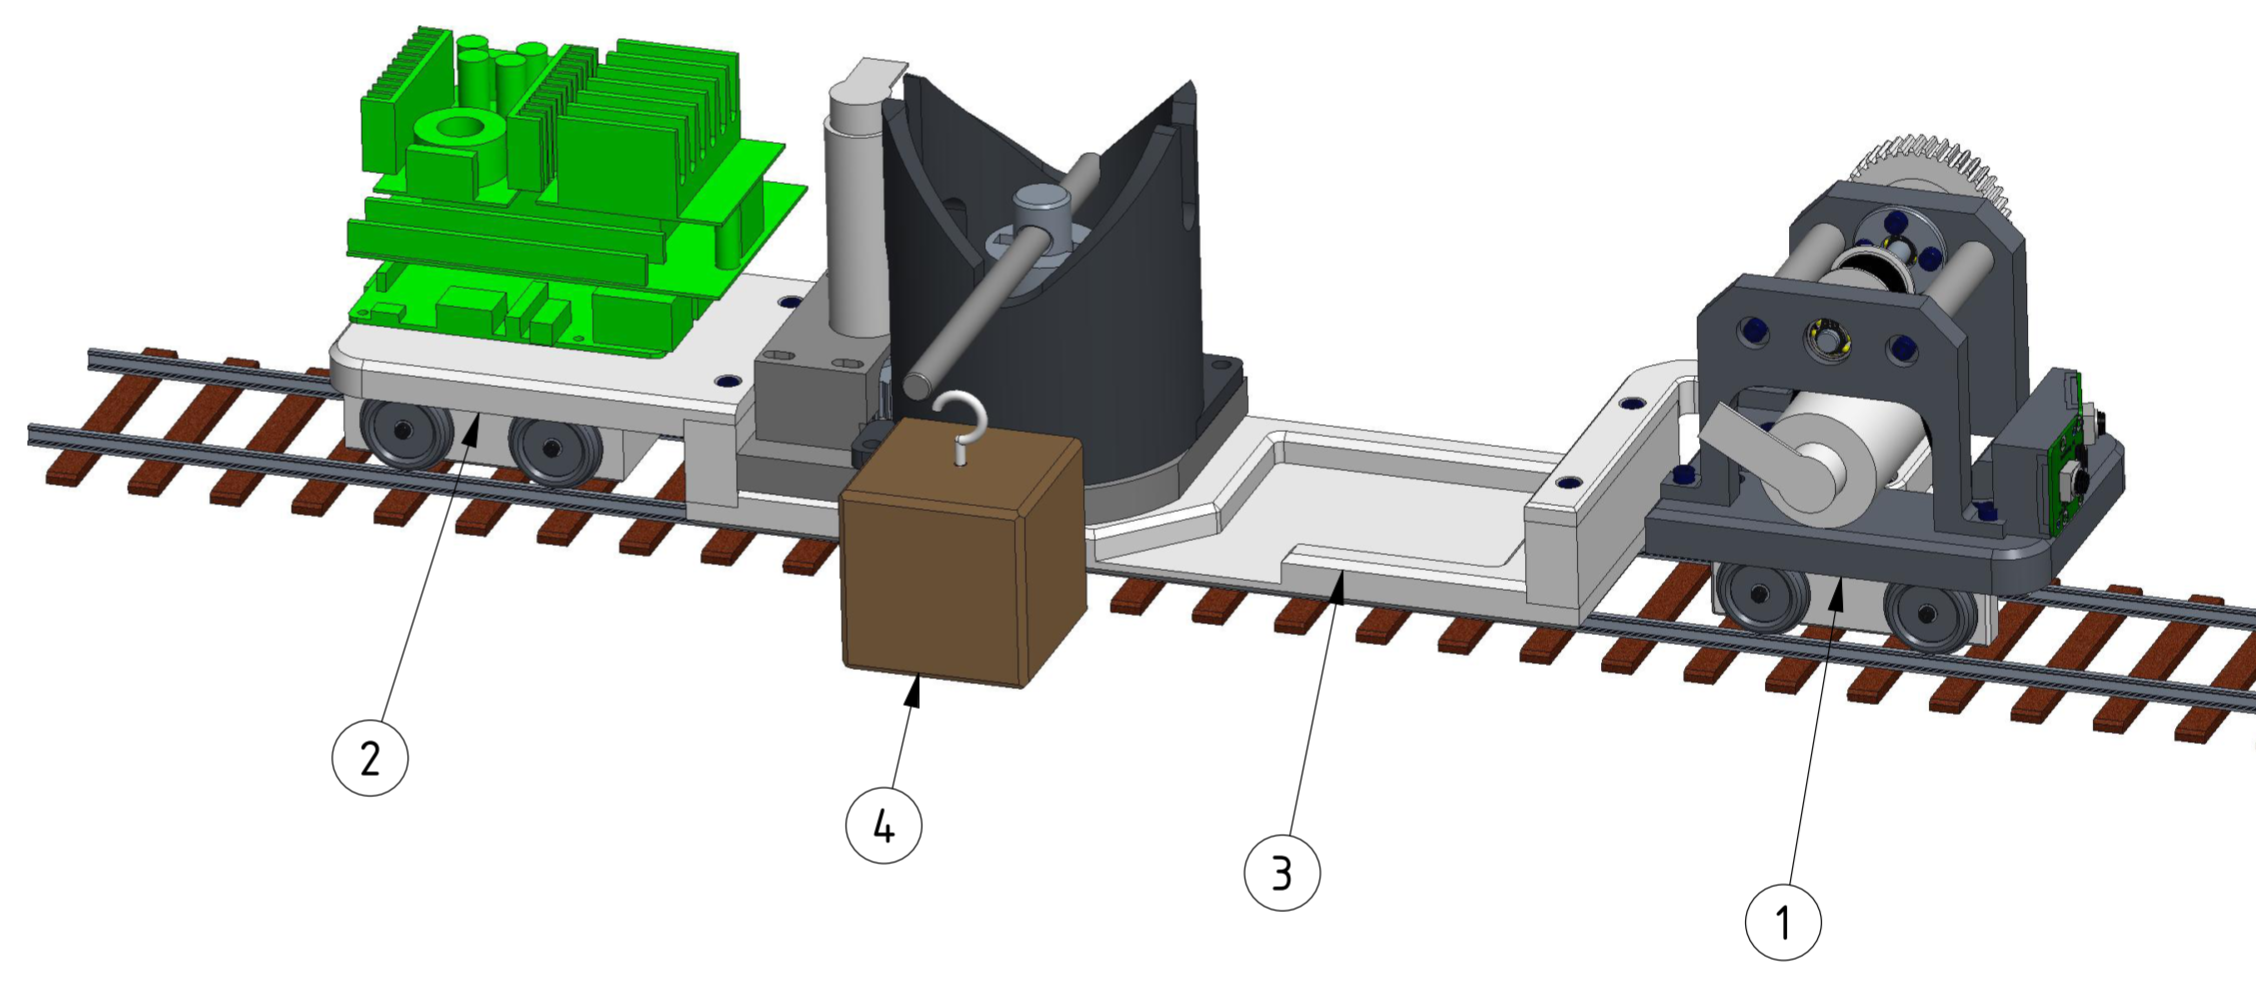
\includegraphics[width=.95\textwidth]{../../images/Maschinentechnik/lokomotive.PNG}
   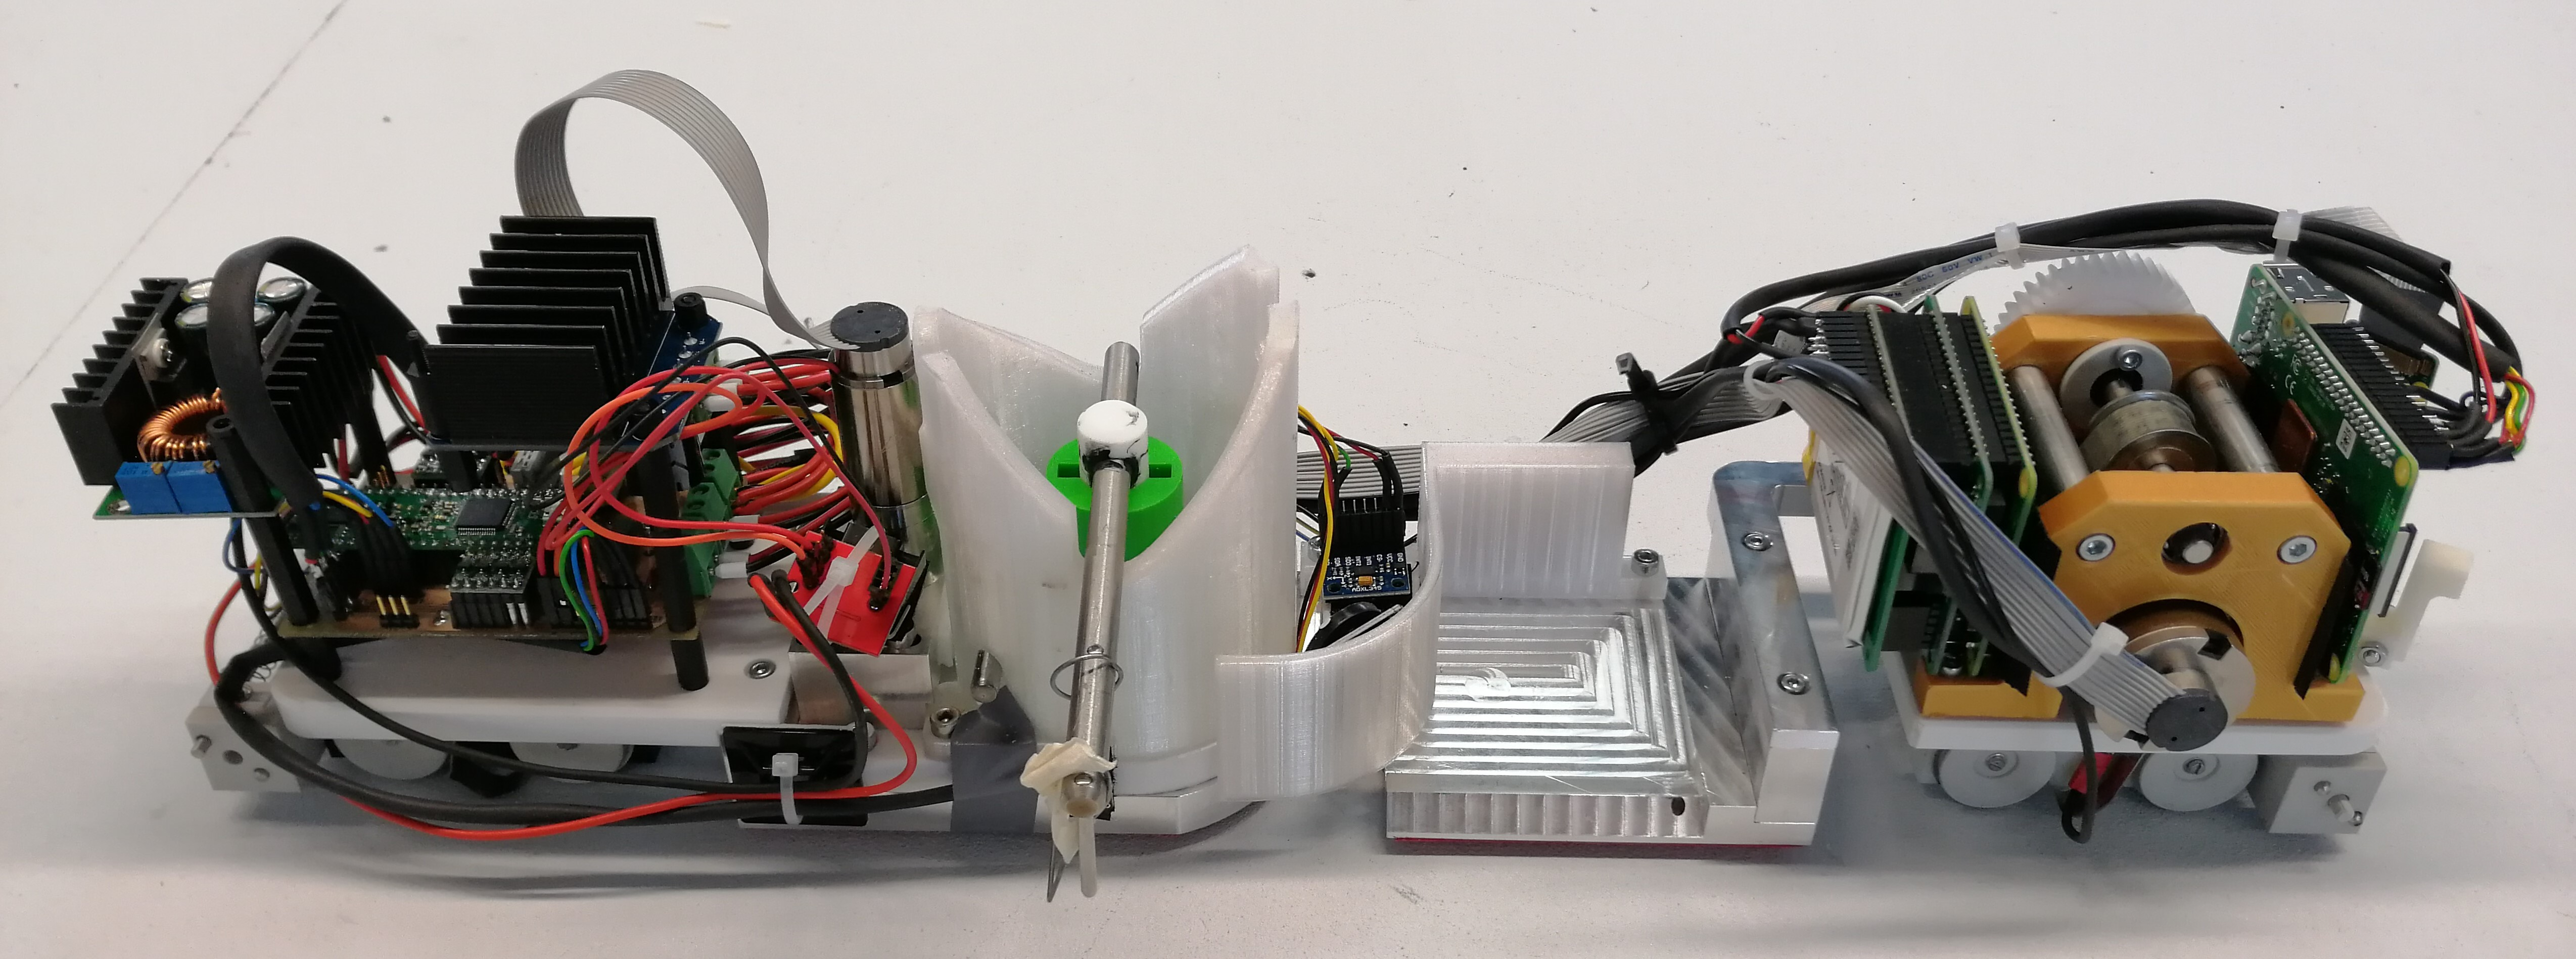
\includegraphics[width=.95\textwidth]{../../images/Maschinentechnik/lokomotive2.PNG}
   \caption {Konzept und Ergebnis des Fahrwerkes}
   \label{fig:konzeptfahrwerk}
\end{figure}

\textbf{Antriebswagen}

Der Antriebswagen (siehe Abbildung \ref{fig:antriebswagen1} bzw. \ref{fig:antriebswagen2}) besteht aus zwei gelagerten Achsen, welche beide durch einen Riemen angetrieben werden. Der Motor treibt ein kleines Getriebe mit einem Übersetzungsverhältnis von 2:1 den Riemen und somit die beiden Achsen an. Der Motor befindet sich in der Mitte des Riemens, mit dem Ziel den Schwerpunkt möglichst tief zu halten. Alle Räder sind mit Schrauben und Unterlagscheiben an den Achsen befestigt, damit ein schneller und einfacher Radwechsel möglich ist. Zwischen den Rädern befindet sich auf beiden Seiten des Wagens je ein Schleifkontakt aus Federblech, welcher mit einer kleinen Vorspannung auf die Gleise drückt. So werden kleine Unhebenheiten auf der Strecke kein Problem für die Stromabnahme. An der Spitze des Wagens befinden sich zwei Kamerhalterungen, welche einstellbar und mit einem Gummipuffer gedämpft sind. Durch einen Bügel und einer Radiallagerung ist der Antriebswagen mit dem Ladungsträger verbunden.\\

\begin{figure}[H]
\begin{minipage}{.6\textwidth}
  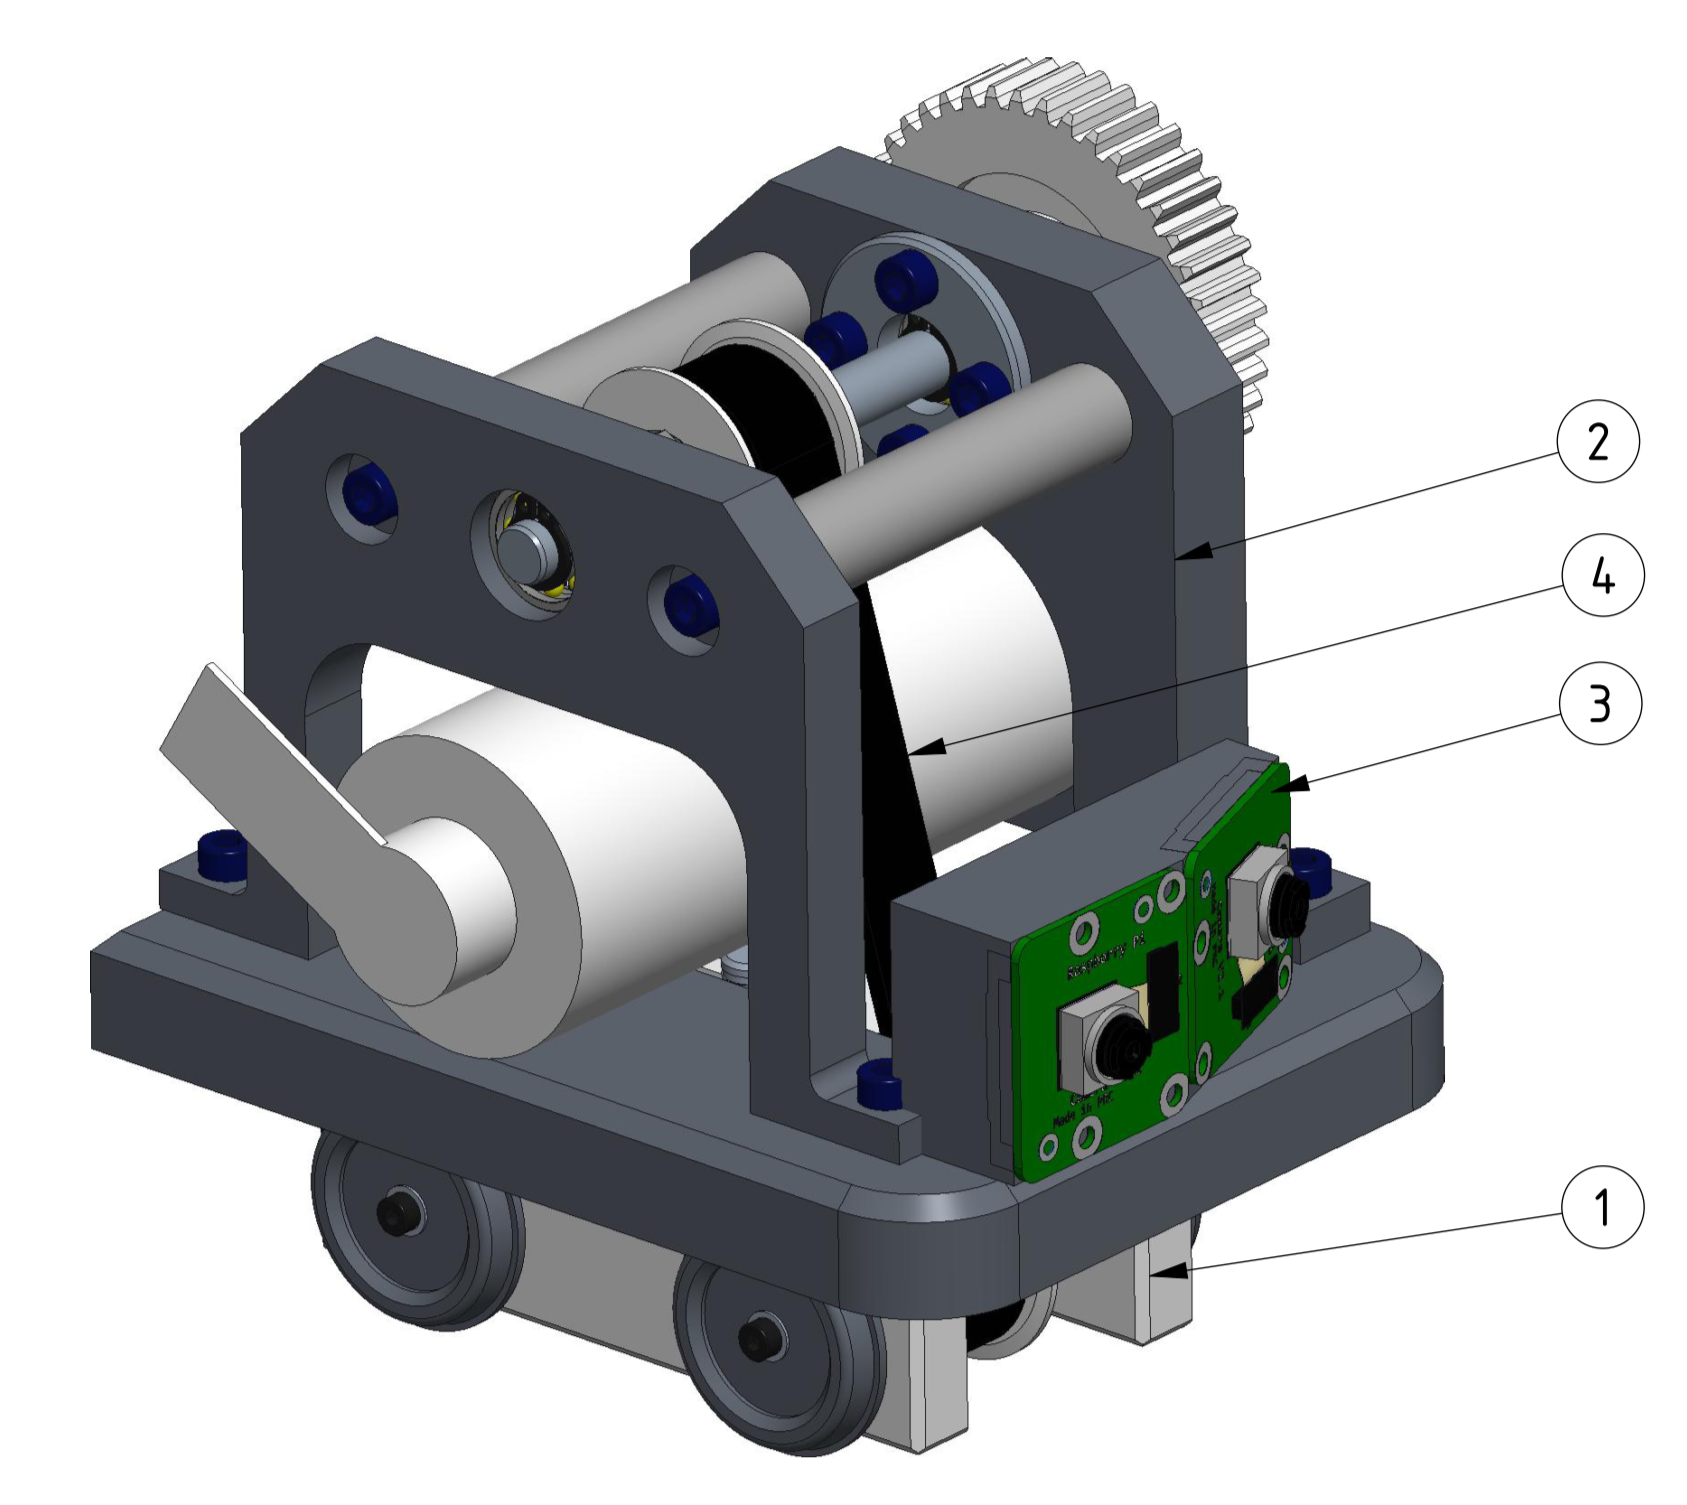
\includegraphics[width=.9\textwidth]{antriebswagen.PNG} 
   \caption[]{Konzept Antriebswagen}
   \label{fig:antriebswagen1}
 \end{minipage}
\begin{minipage}{.4\textwidth}
\begin{table}[H] \centering
  \begin{tabular}{|l|l|}
  \hline
  \textbf{Position} & \textbf{Bezeichnung}\\
  \hline
  Position 1          & Wagen\\
   \hline
  Position 2          & Antriebseinheit\\
  \hline
  Position 3          & Kameras\\
  \hline
  Position 4          & Zahnriemen\\
  \hline
 \end{tabular}
 \caption{Positionsnummern}
 \label{tab:expl_antriebswagen}
 \end{table} 
 \end{minipage} 
\end{figure} 

\begin{figure}[H]
    \centering
    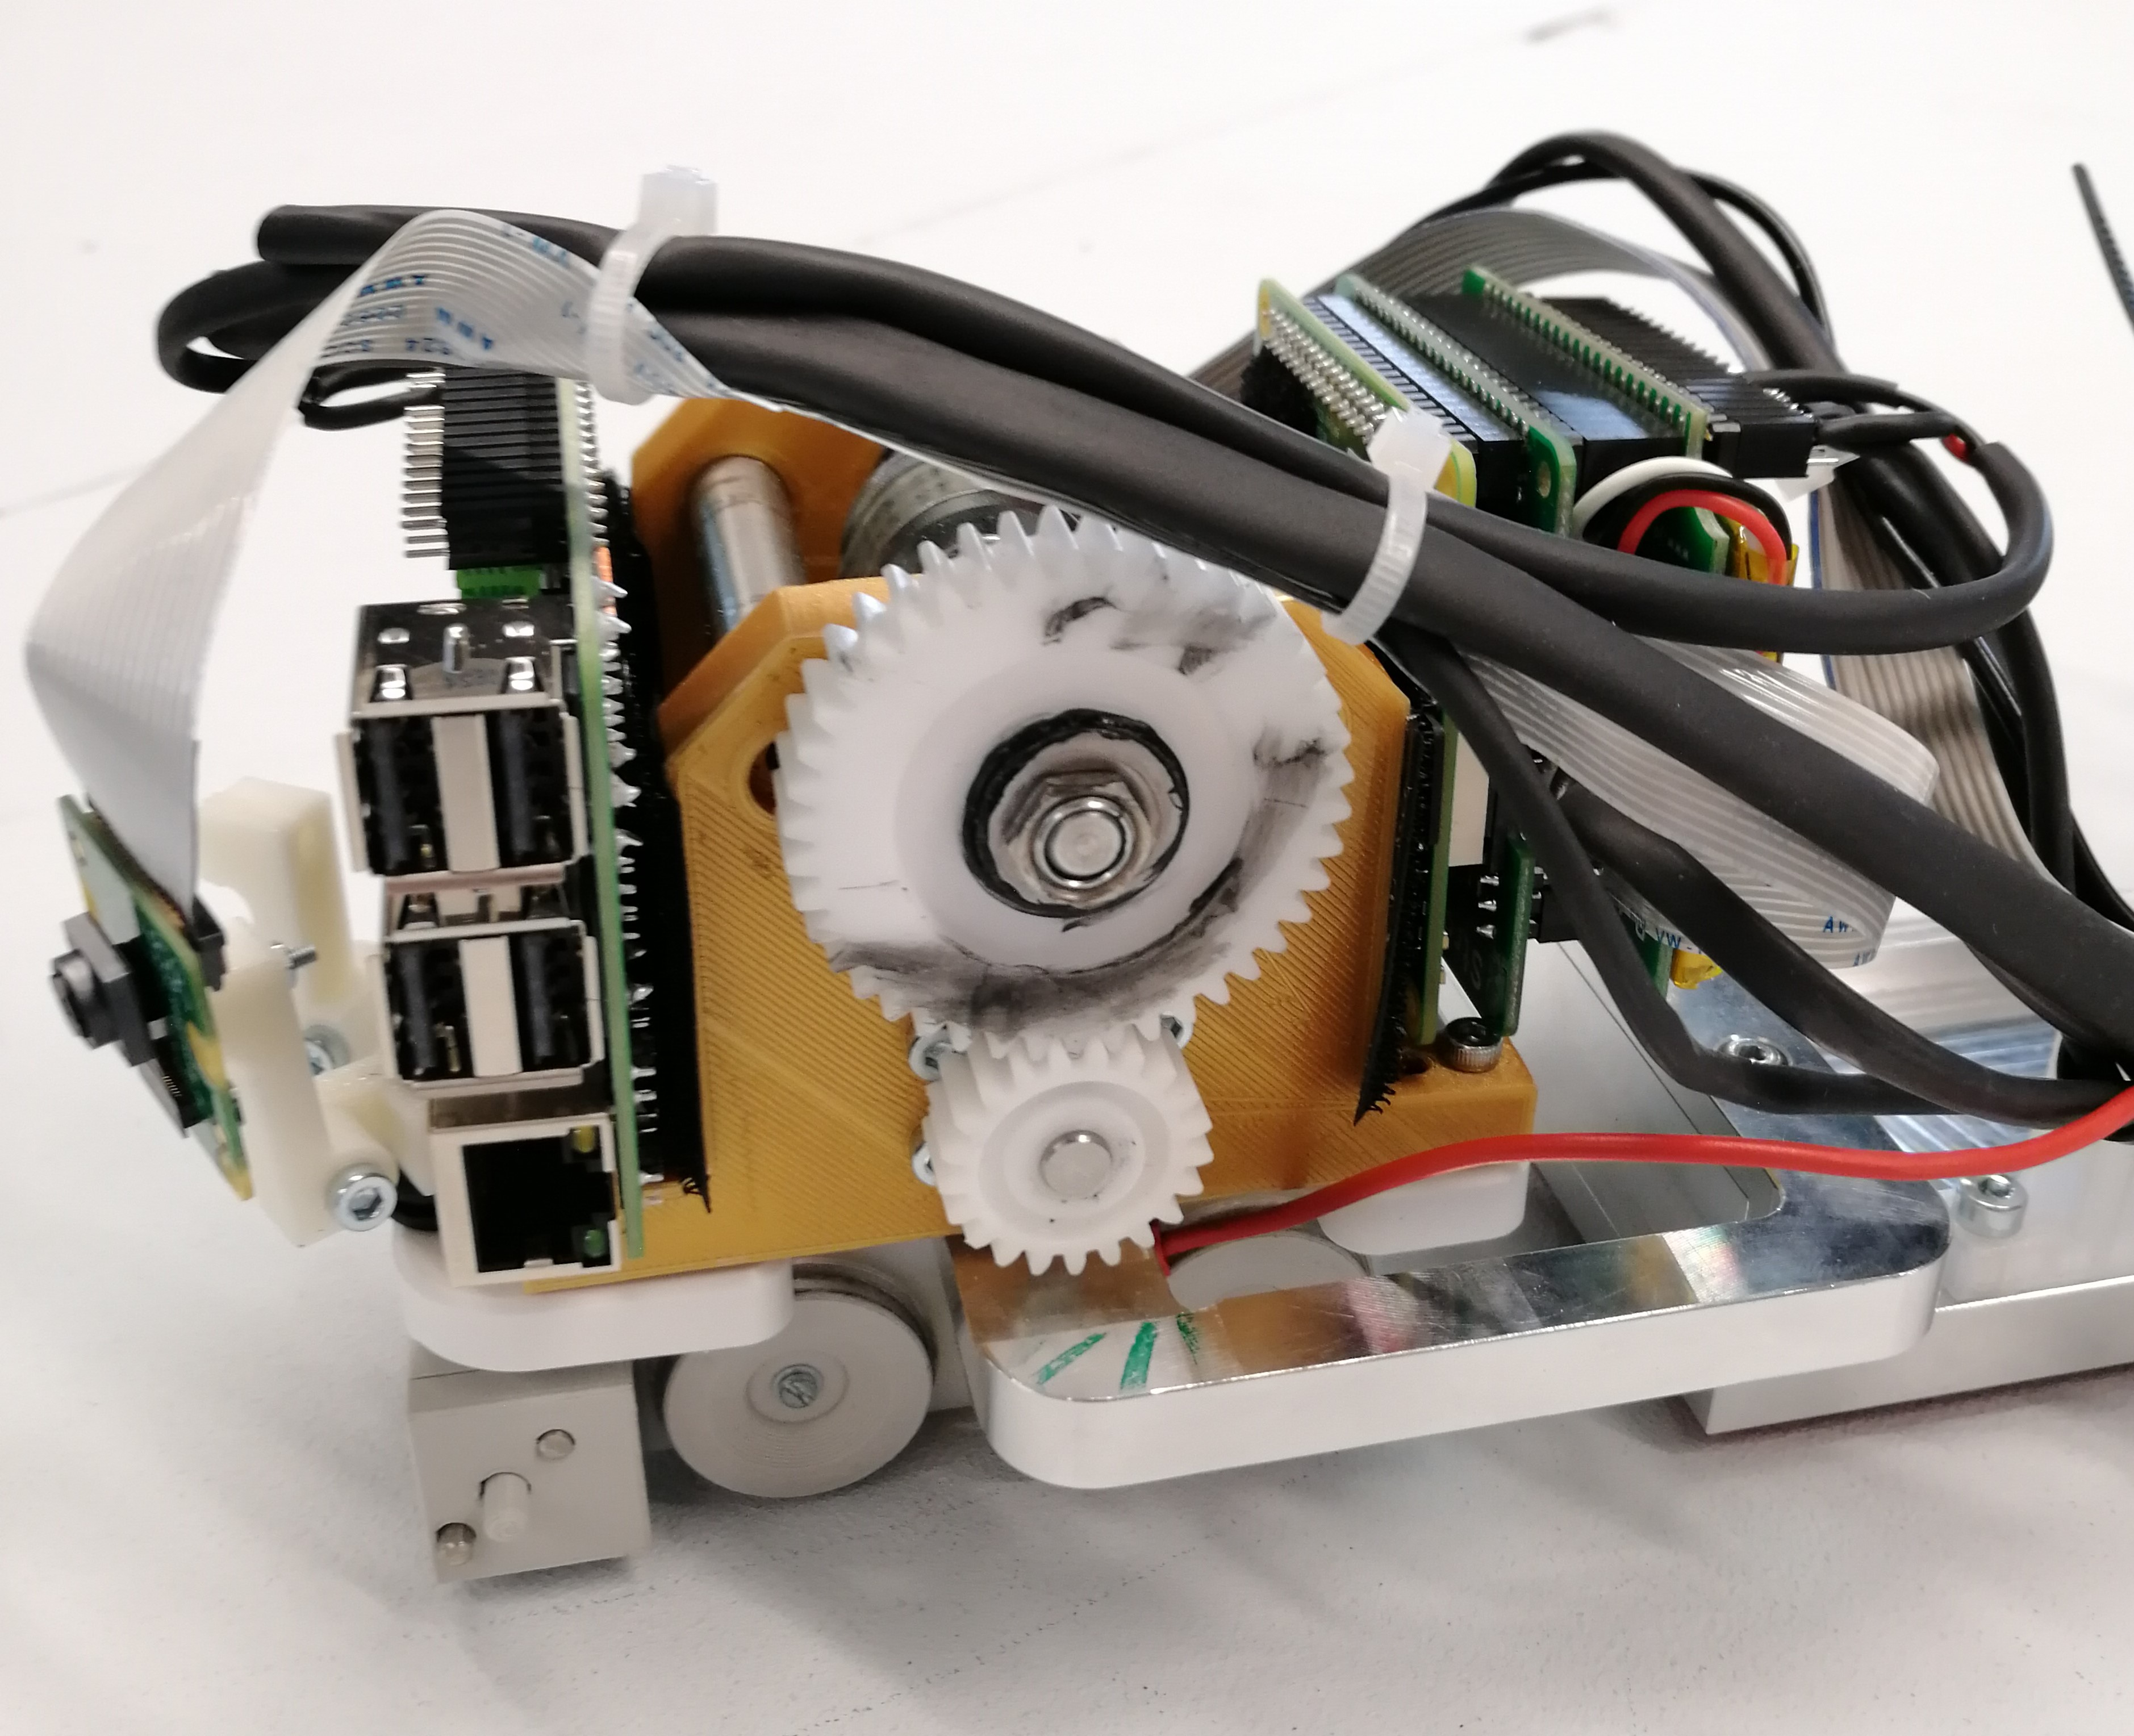
\includegraphics[width=0.495\textwidth]{../../images/Maschinentechnik/antriebswagen3.PNG}
    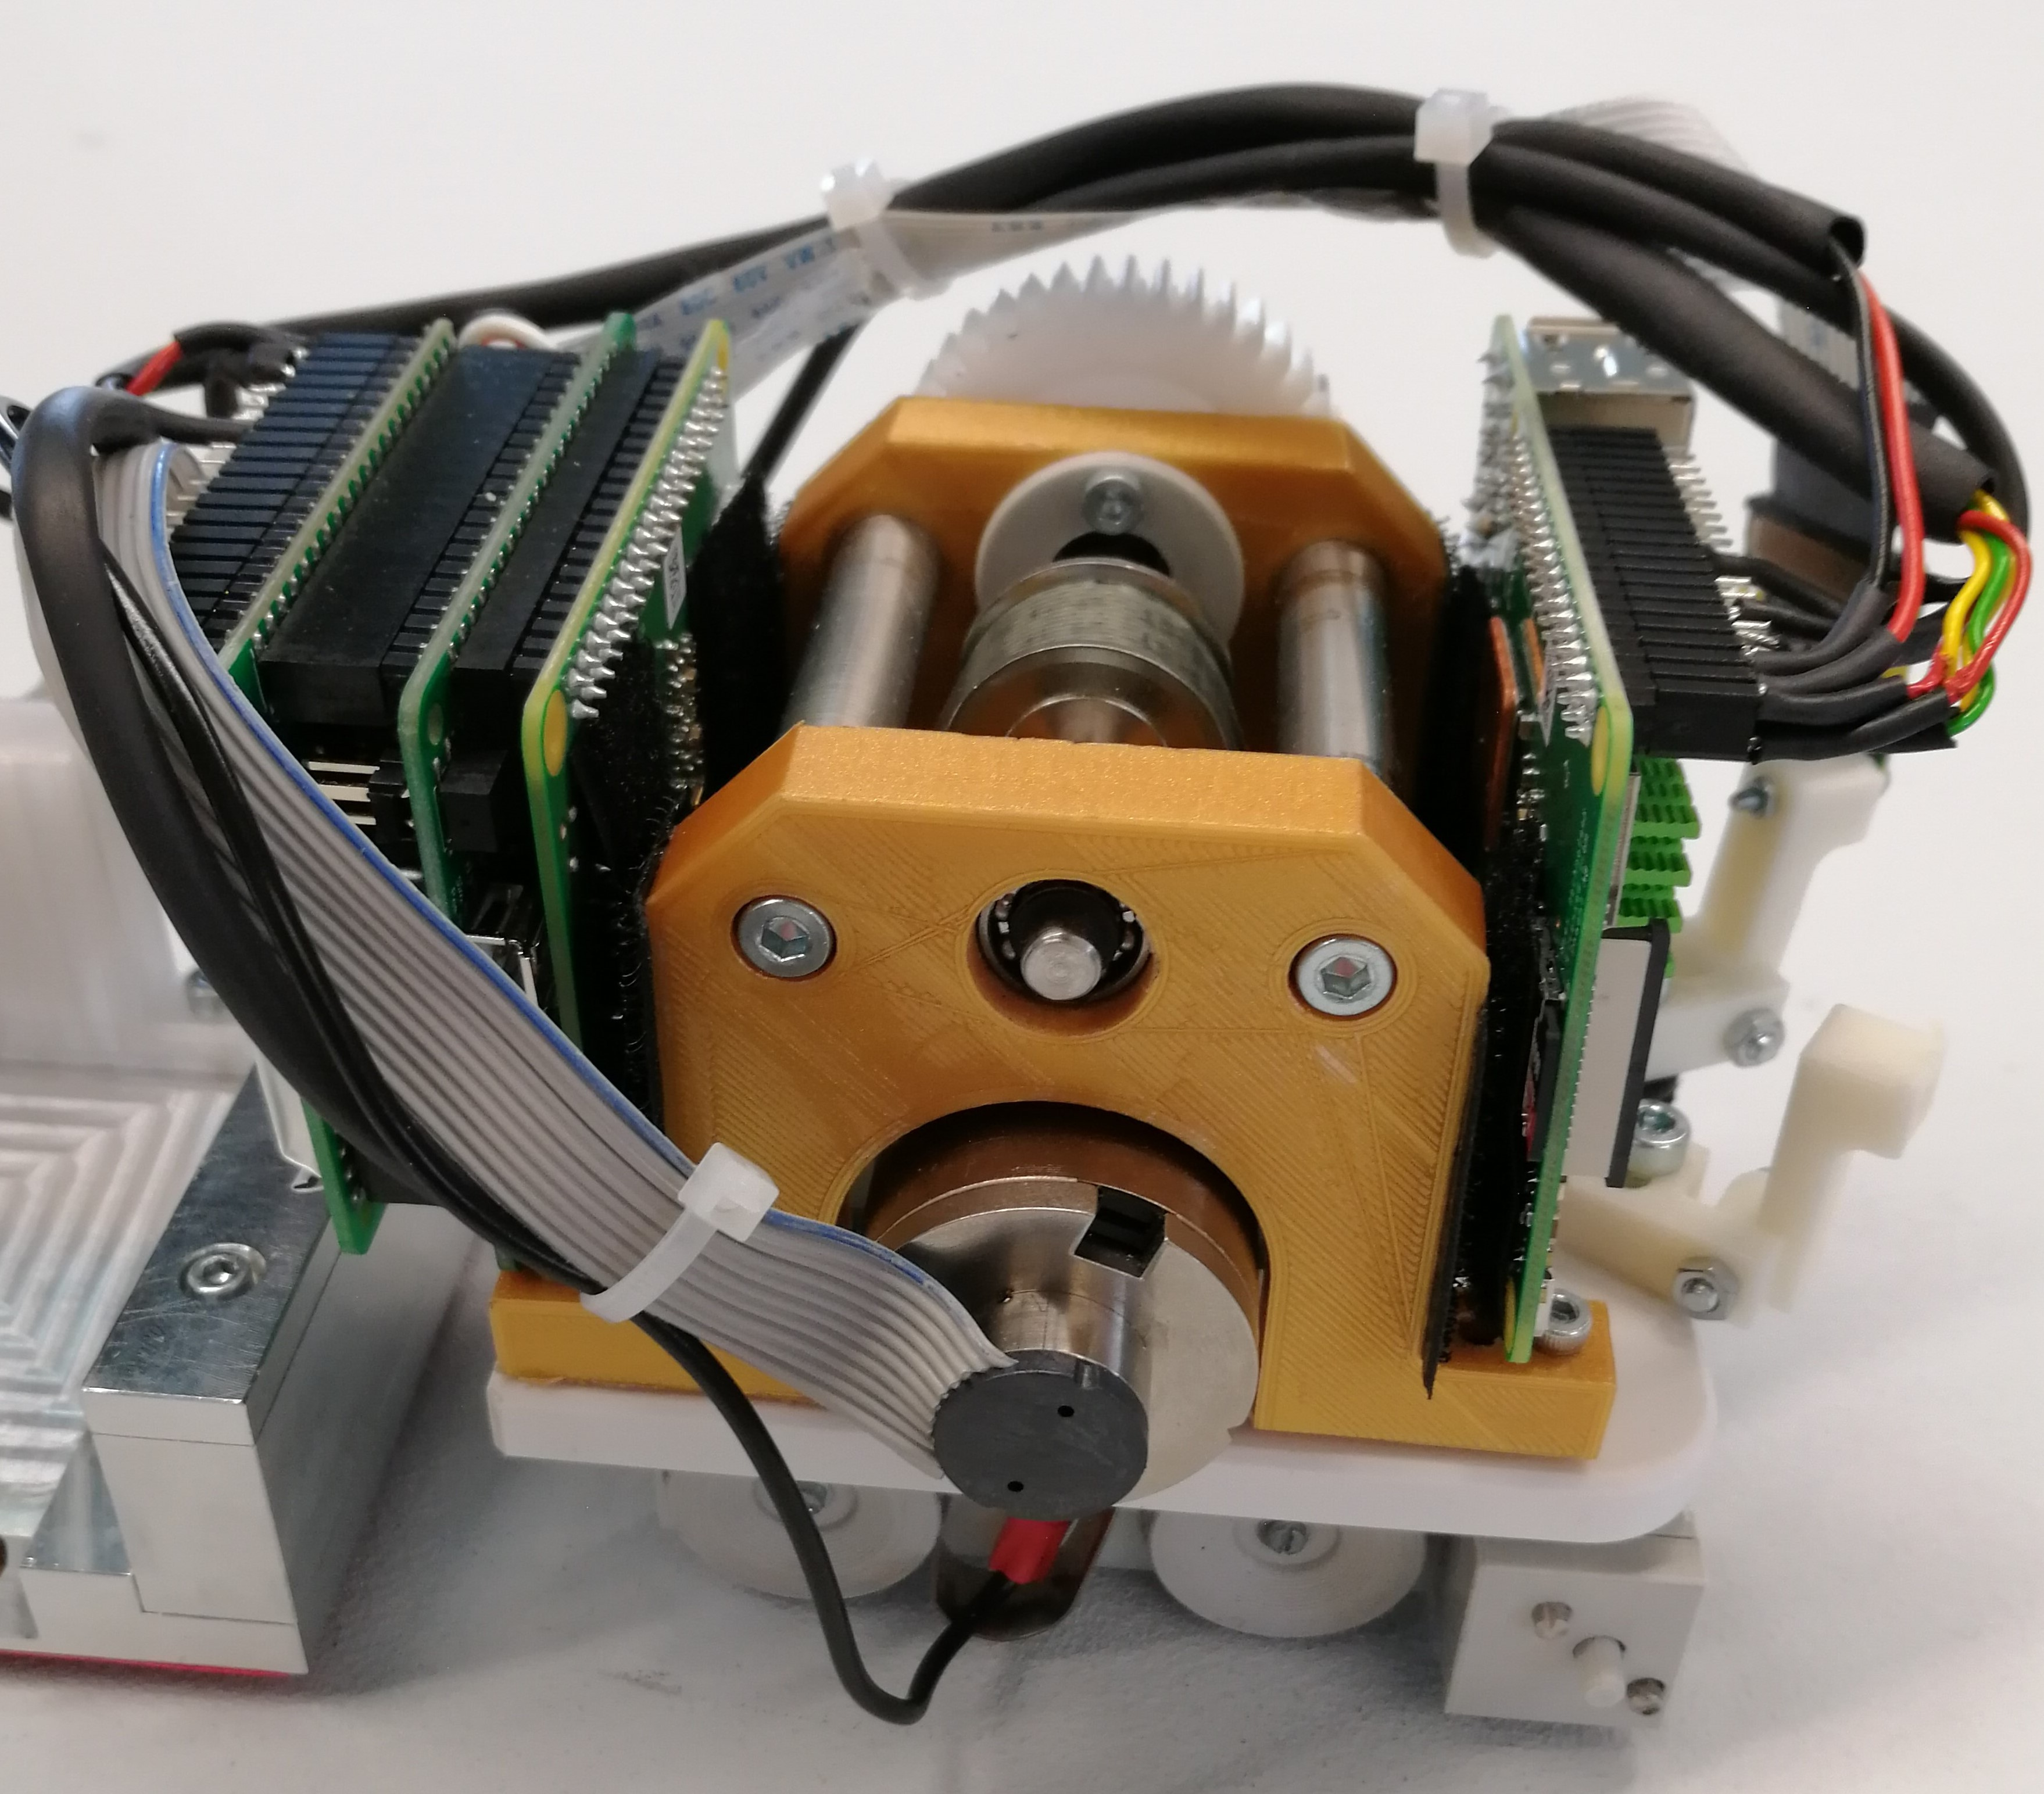
\includegraphics[width=0.455\textwidth]{../../images/Maschinentechnik/antriebswagen4.PNG}
    \caption {Antriebswagen Endprodukt}
    \label{fig:antriebswagen2}
\end{figure}

Direkt unterhalb der Kamerahalterung befindet sich eine Kurvenvorrichtung (siehe Abbildung \ref{fig:kurvenvorrichtung}), welche die Gefahr des Entgleisens des Zuges minimiert. Sie funktioniert folgendermassen: Durch zwei Stahlstifte, welche radial die Kontur des Gleises haben und drehbar gelagert sind wird die Lokomotive in der Spur geführt. Die beiden Federn sorgen für den nötige Anpressdruck, damit die Vorrichtung in die Gleise verkeilt wird.\\

\begin{figure}[H]
  \centering
  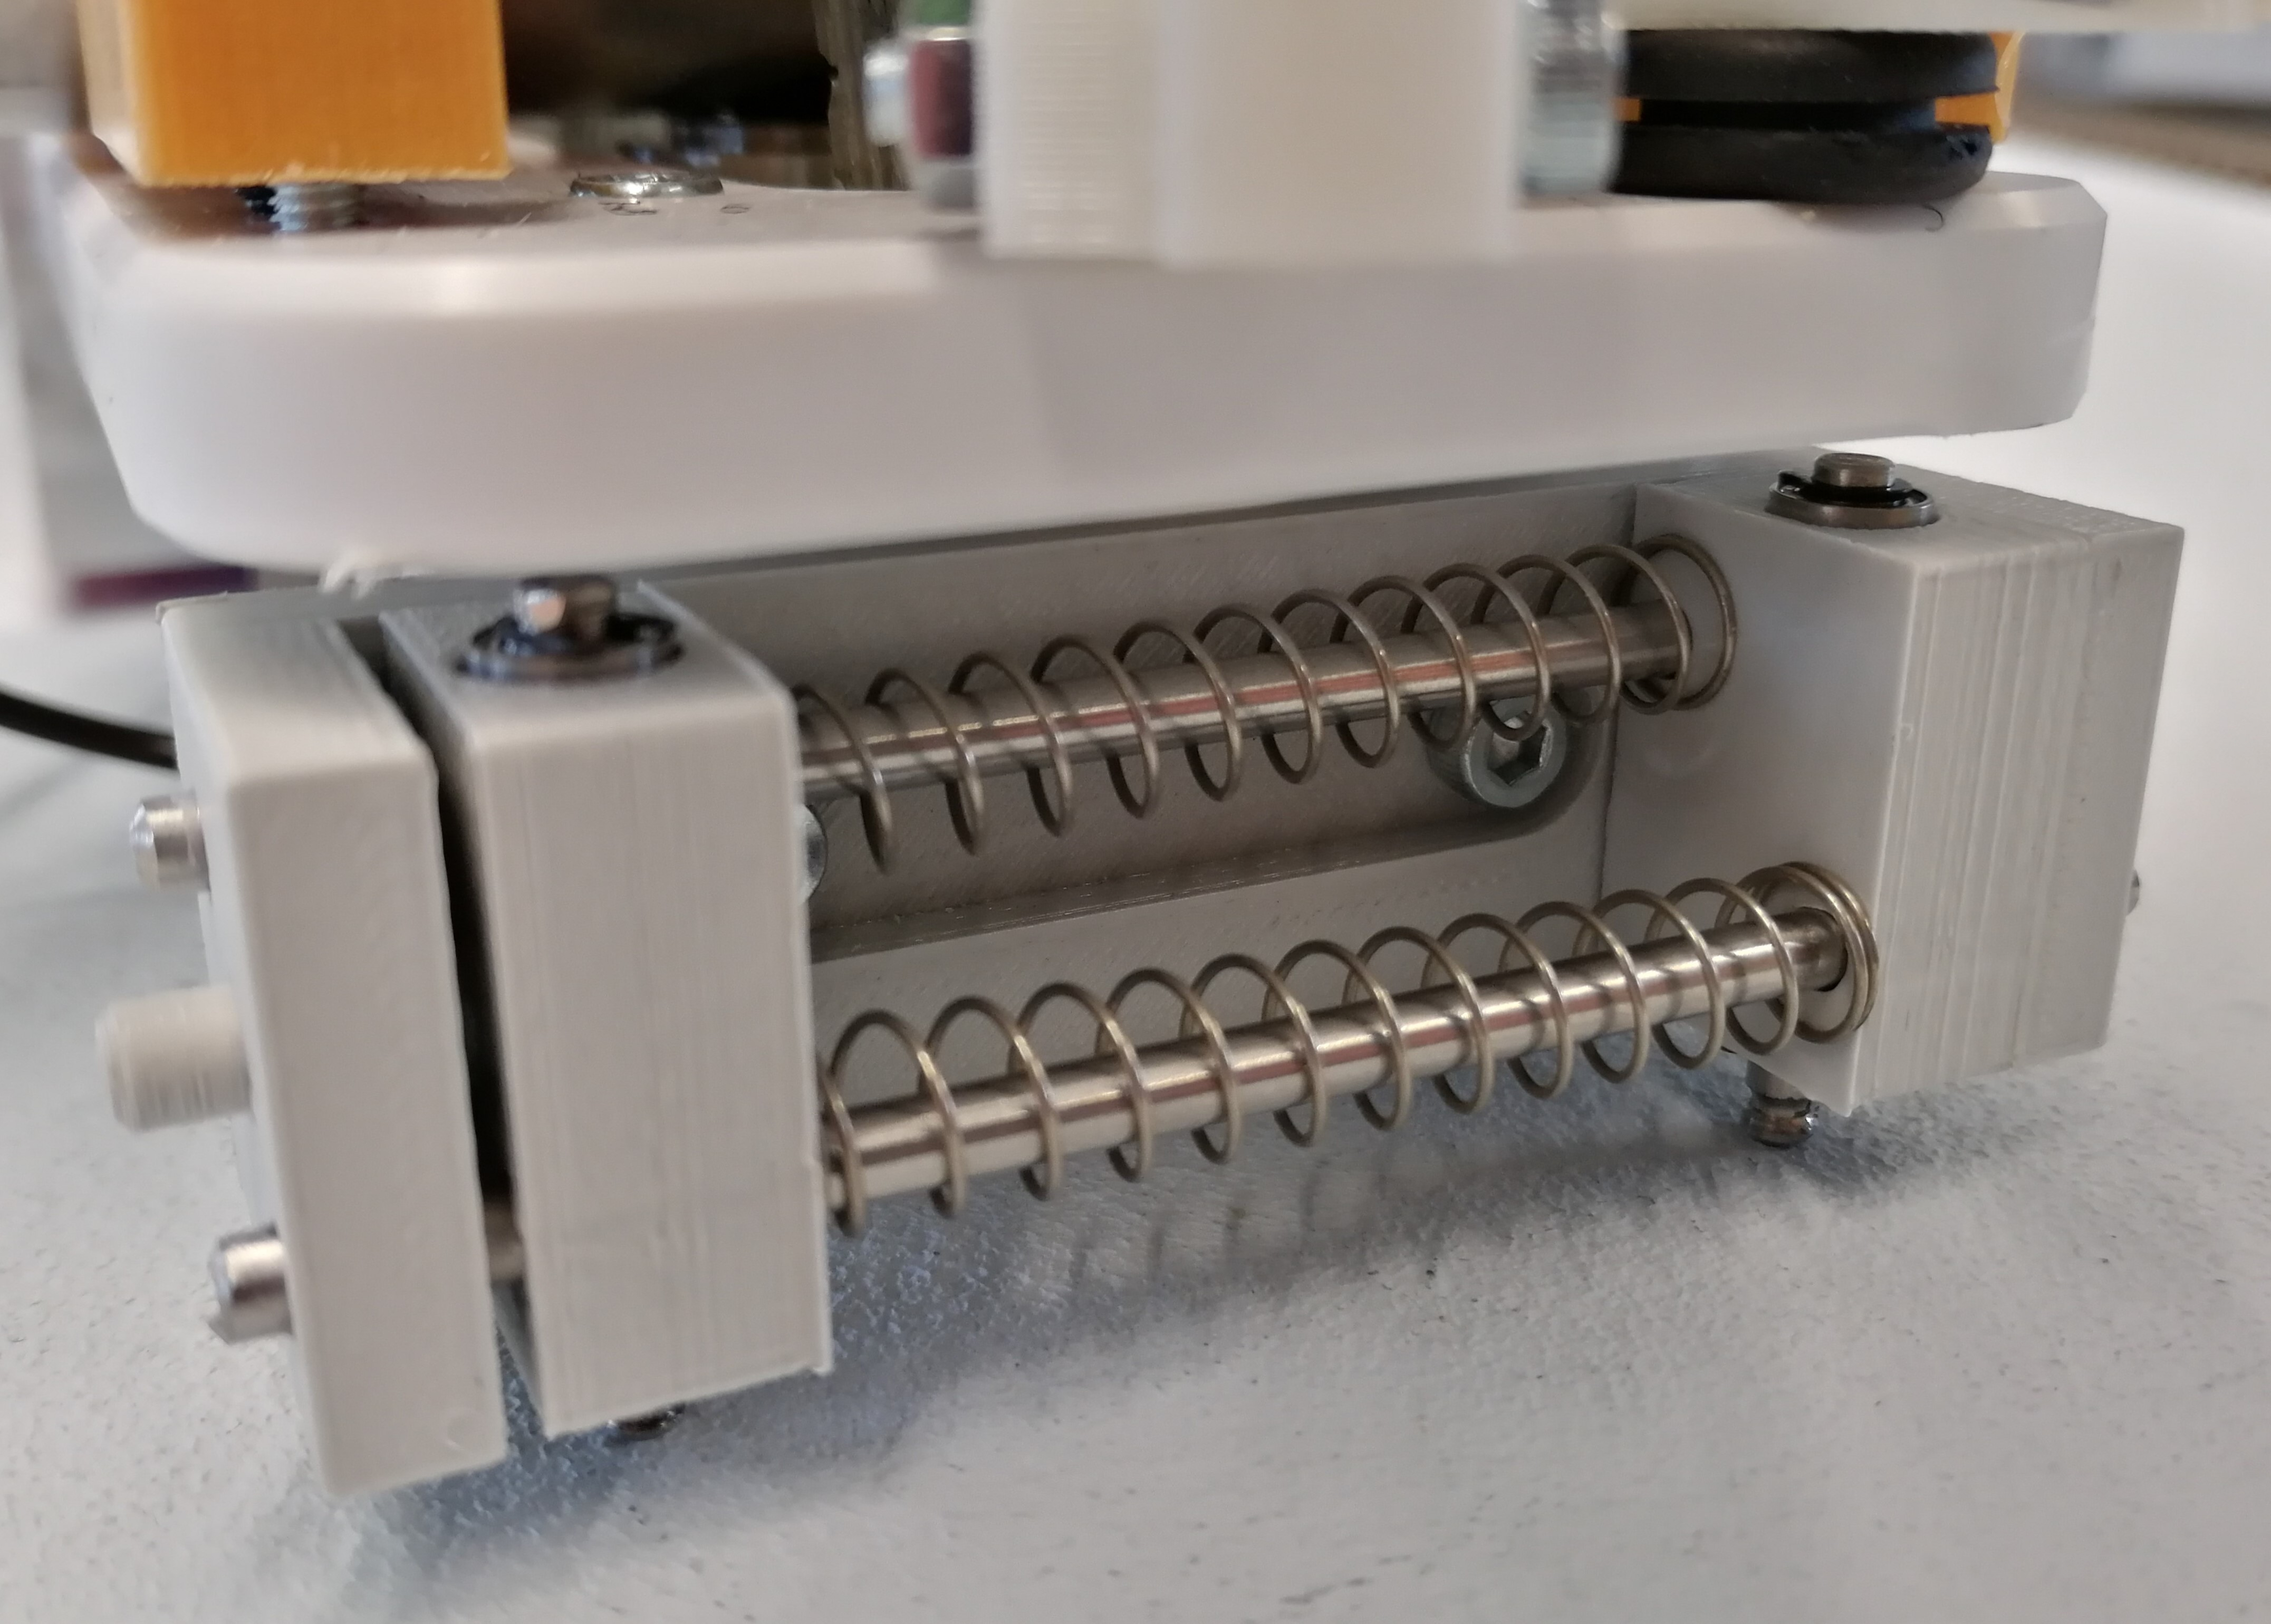
\includegraphics[width=0.37\textwidth]{../../images/Maschinentechnik/kurvenvorrichtung.PNG}
  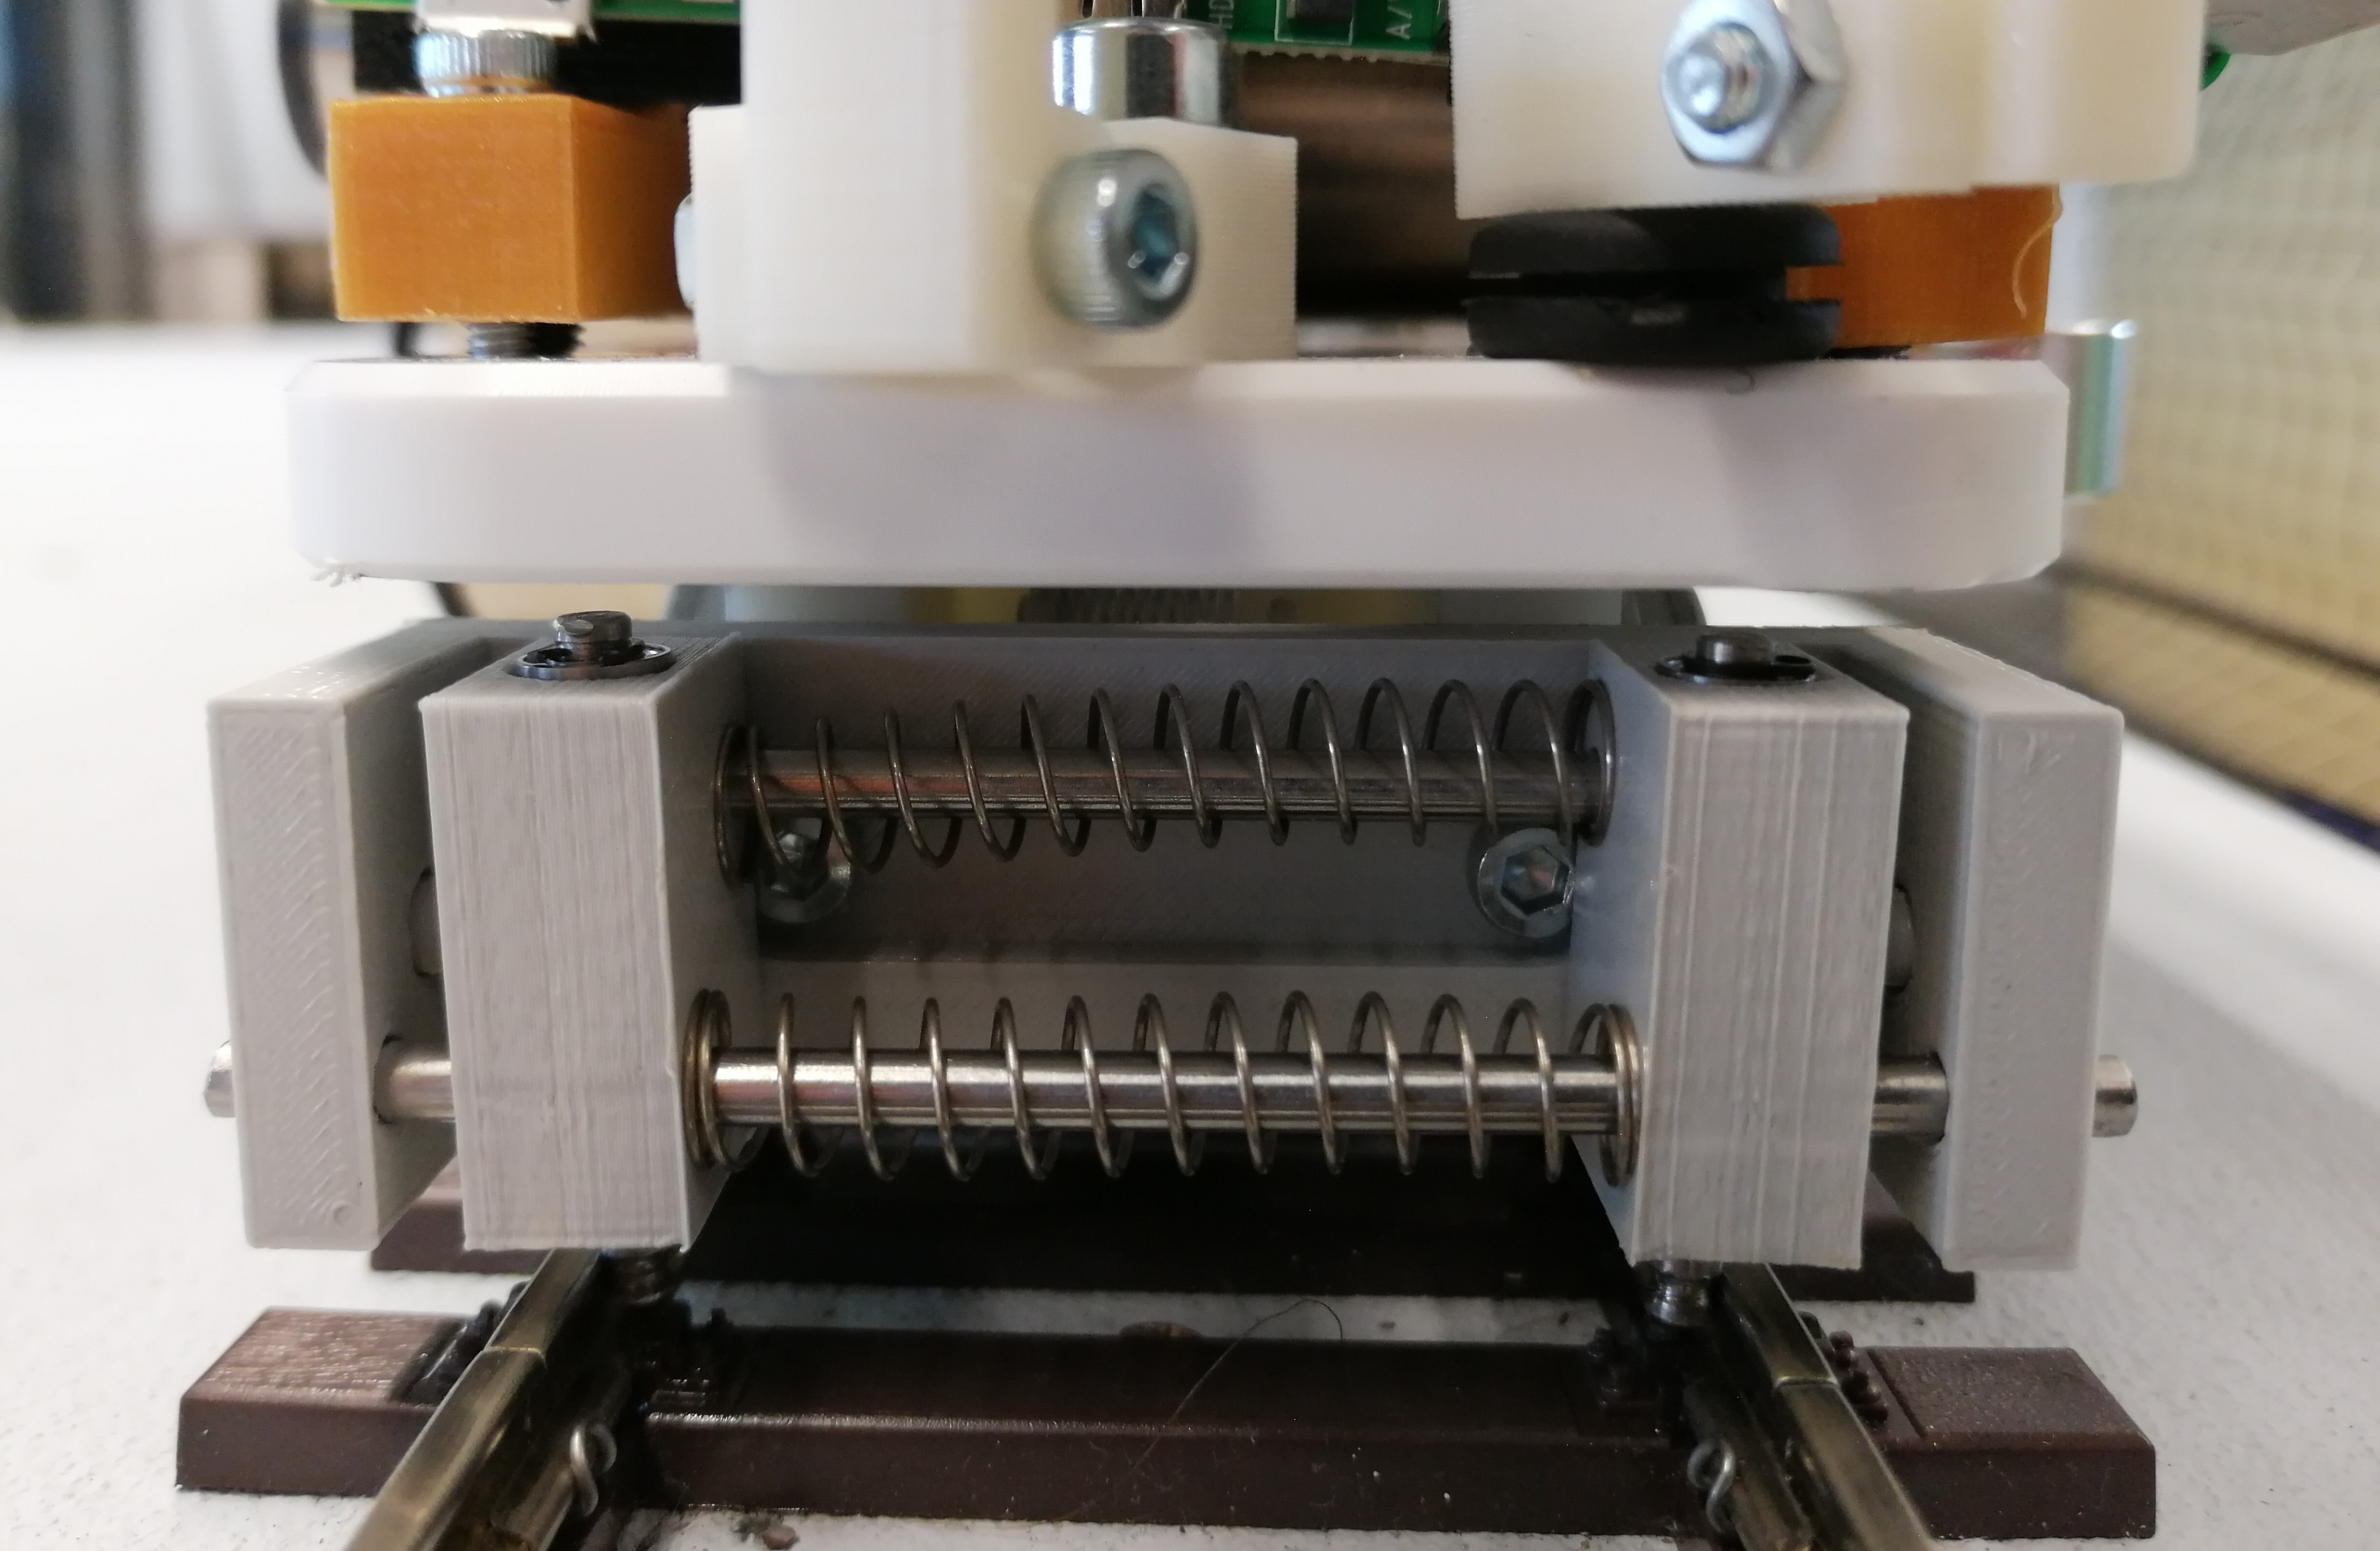
\includegraphics[width=0.4\textwidth]{../../images/Maschinentechnik/testkurvenvorrichtung2.PNG}
  \caption {Kurvenvorrichtung in unmontiertem und montiertem Zusatand}
  \label{fig:kurvenvorrichtung}
\end{figure}

\pagebreak

\begin{figure}[H]
  \begin{minipage}{.5\textwidth}
    \textbf{Führungwagen}\\
    Der Führungswagen in Abbildung \ref{fig:fuehrungswagen1} ist grundsätzlich gleich aufgebaut wie der Antriebswagen. Er hat zwei gelagerte Achsen, an welchen je zwei Räder mit Schrauben und Unterlagscheiben befestigt sind. Zwischen den Rädern hat es jeweils einen Schleifkontakt aus Federstahl, welcher auf die Gleise vorgespannt ist und den Strom somit an einer zweiten Stelle vom Gleis abnimmt. Am hinteren Ende des Führungswagen befindet sich wiederum die Vorrichtung für die Kurvenfahrt. Durch einen Stift und ein Radiallager ist der Ladungsträger mit dem Führungswagen schwenkbar verbunden.
   \end{minipage}
  \begin{minipage}{.5\textwidth}
    \flushright
    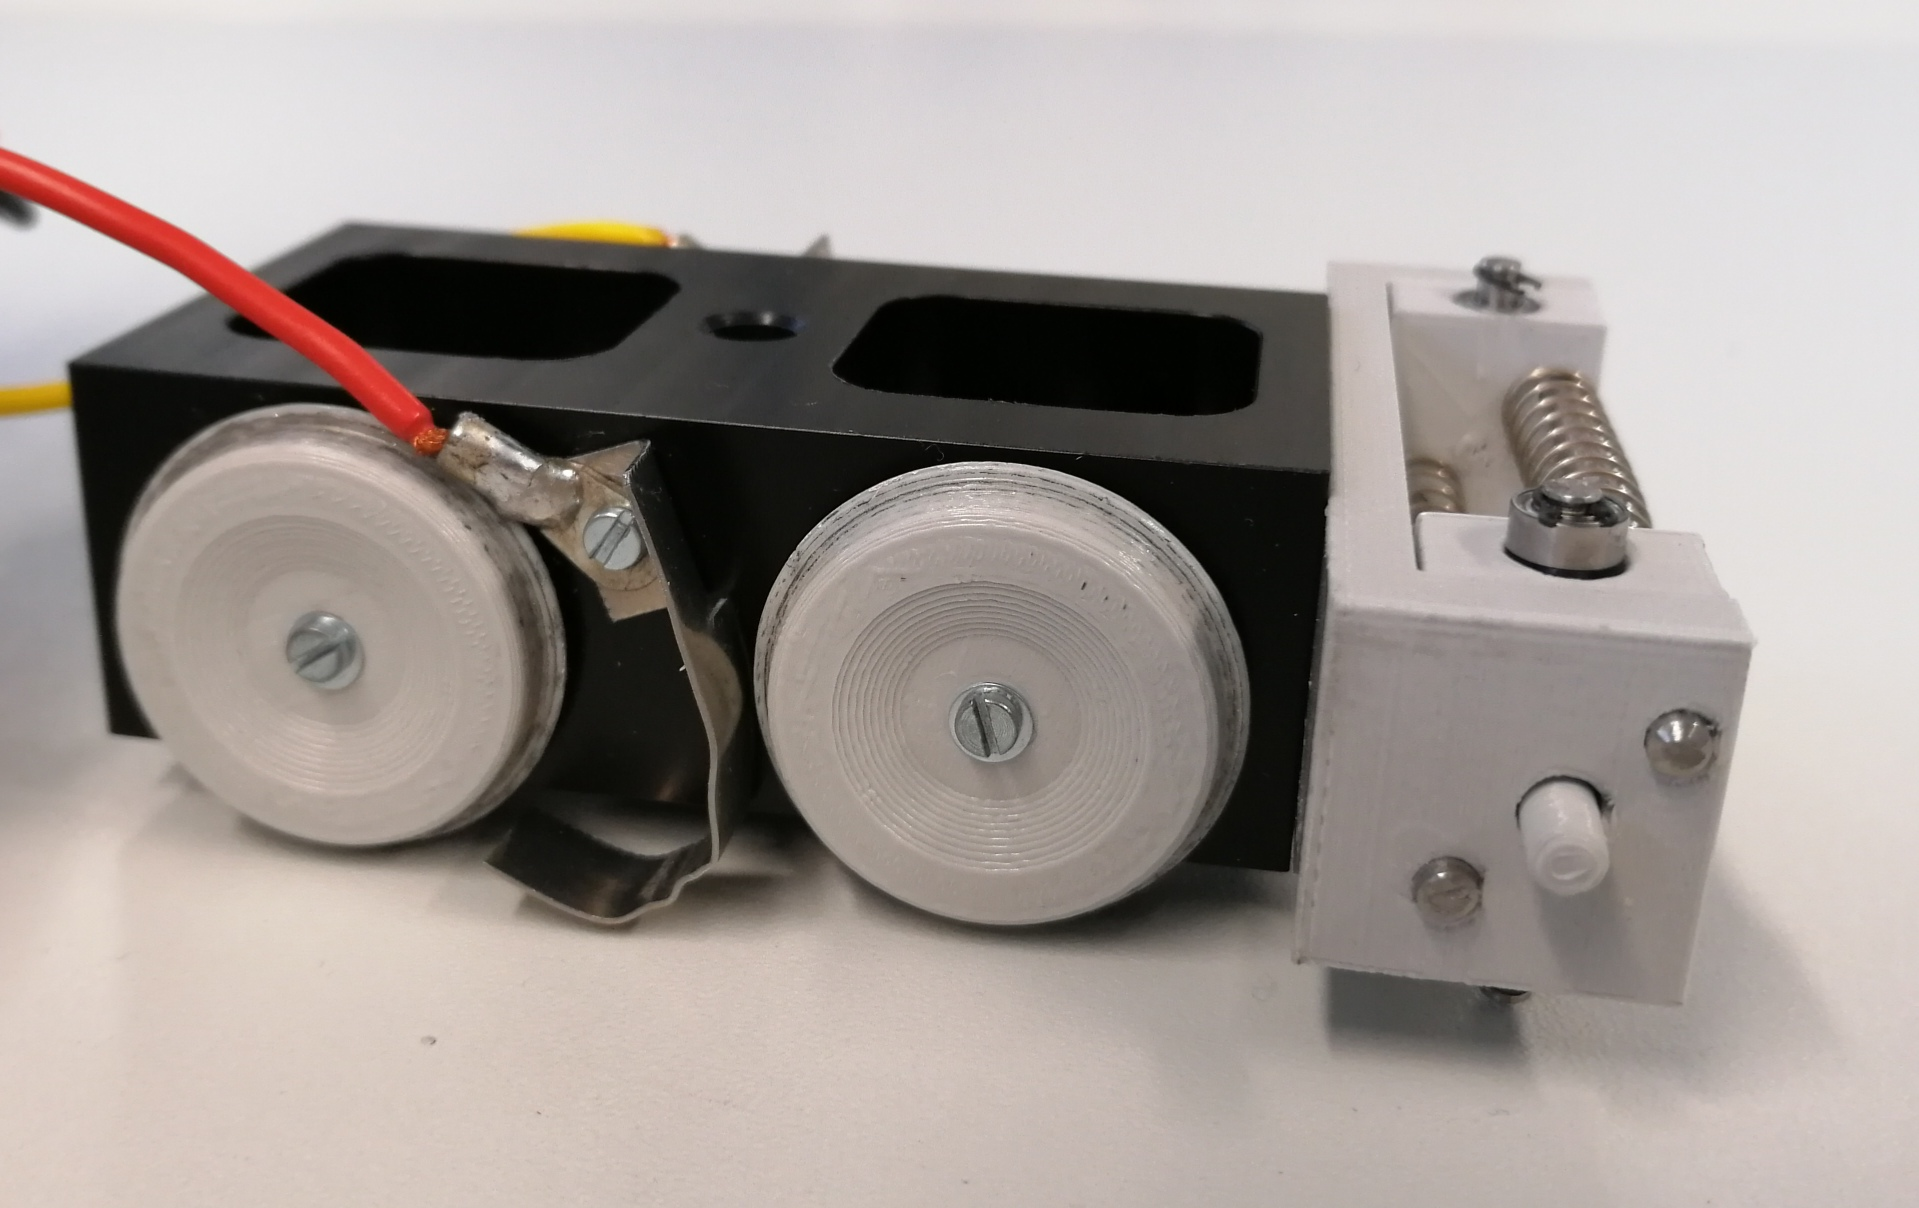
\includegraphics[width=0.95\textwidth]{fuehrungswagen2.JPG}
    \caption {Führungswagen}
    \label{fig:fuehrungswagen1}
    \end{minipage} 
\end{figure} 

Der Aufbau des Führungswagens ist wie konzipiert, mit Ausnahme der Räder, finalisiert und hergestellt worden. Der Führungswagen ist folgendermassen aufgebaut:\\

\begin{figure}[H]
  \centering
  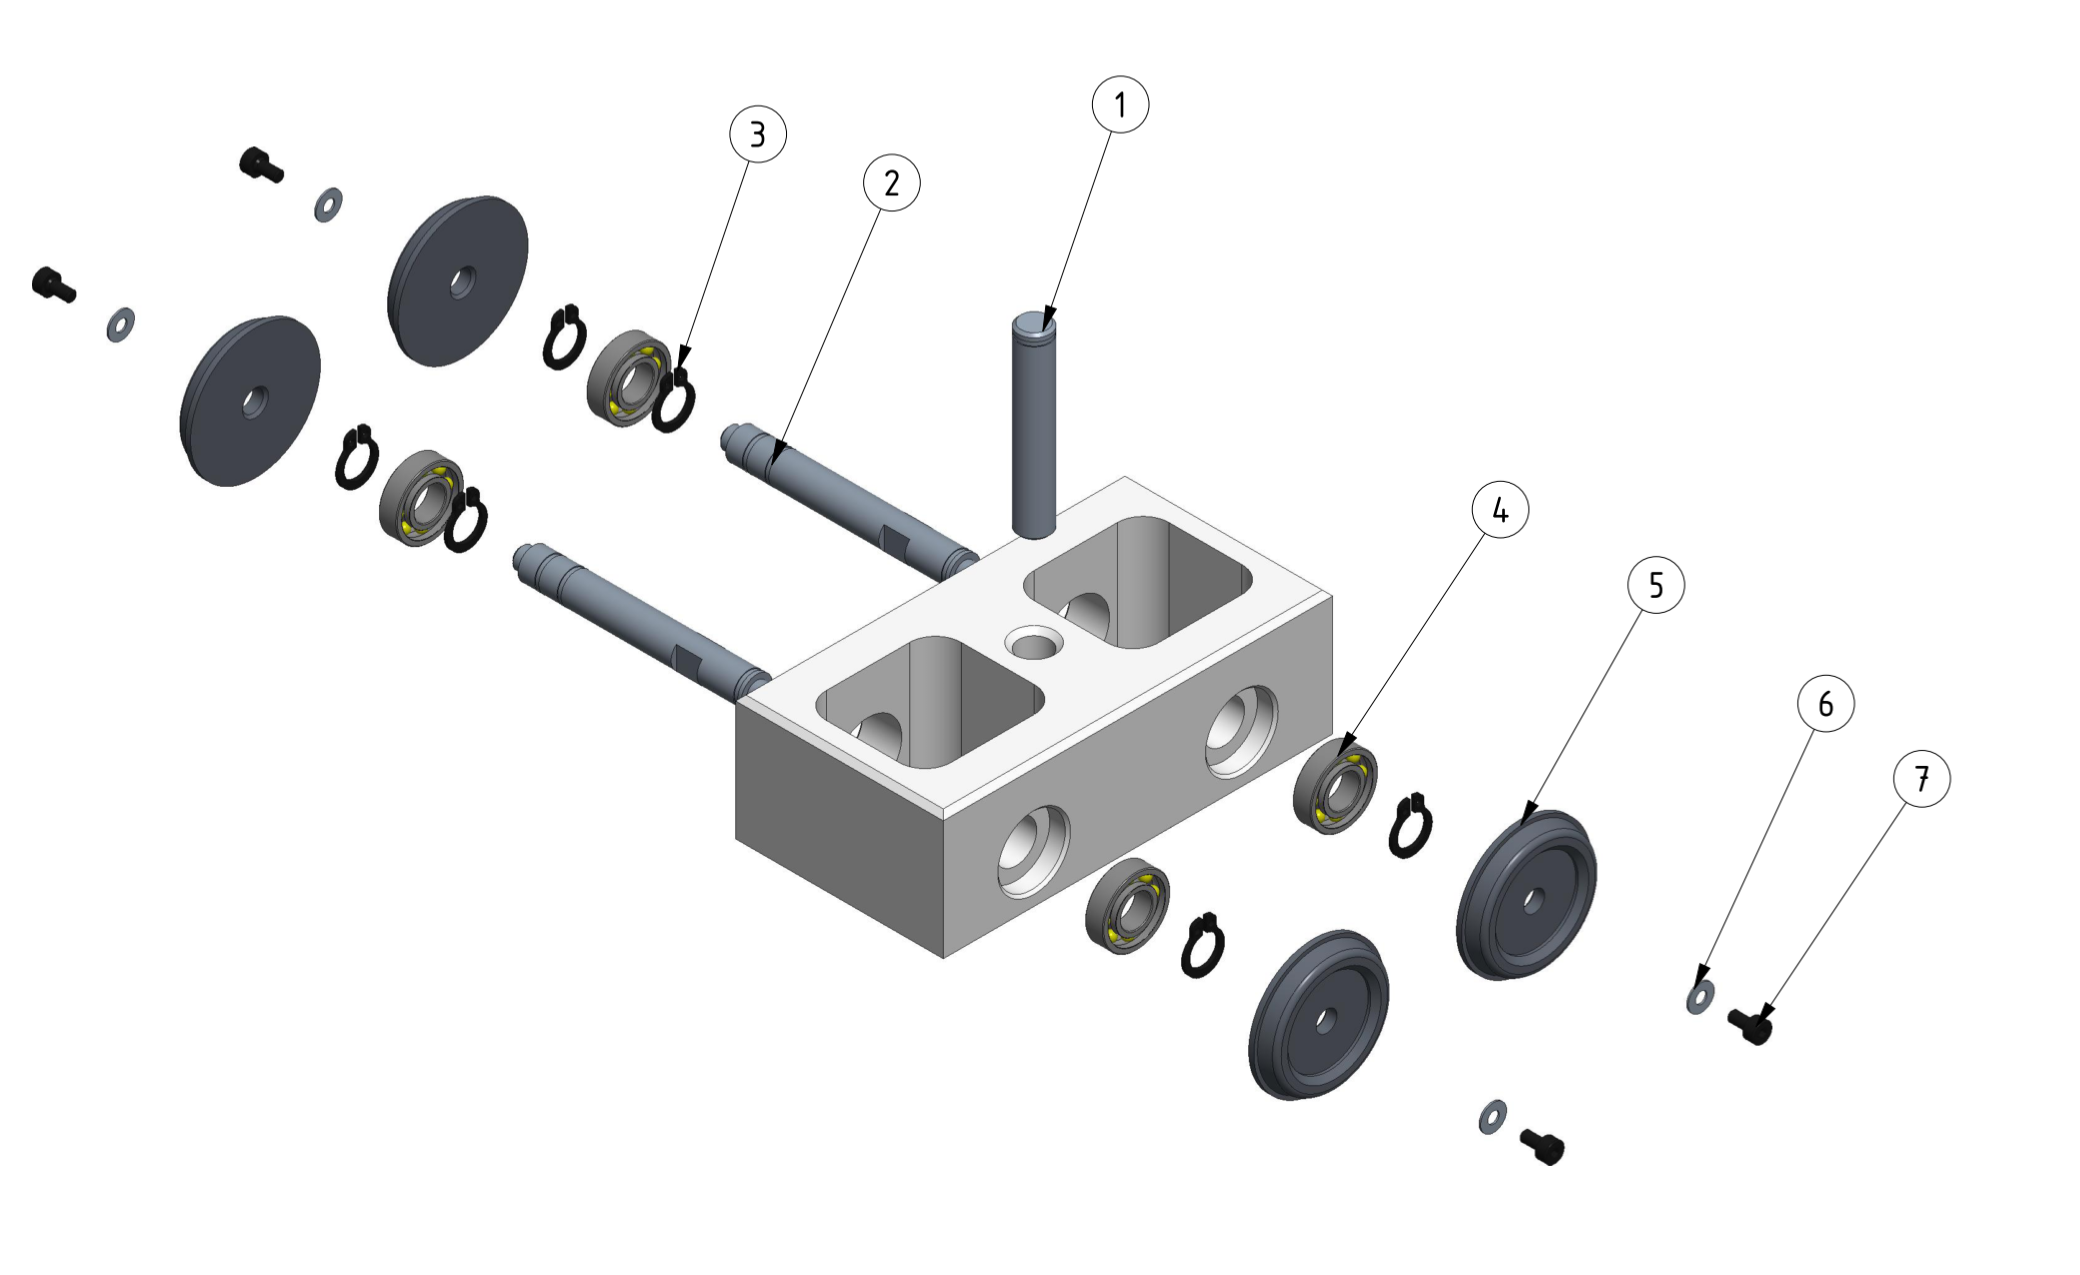
\includegraphics[width=0.7\textwidth]{fuehrungswagen.PNG}
  \caption {Konzept des Führungswagens}
  \label{fig:fuehrungswagen2}
\end{figure}

\begin{table}[H] \centering
  \begin{tabular}{|l|l|}
  \hline
  \textbf{Position} & \textbf{Bezeichnung}\\
  \hline
  Position 1          & Drehachse Wagen-Ladungsträger (eingepresst)\\
   \hline
  Position 2          & Achsen (Gewinde an beiden Seiten, Anfräsfläche für Gabelschlüssel)\\
   \hline
  Position 3          & Sicherungsring für Rillenkugellager\\
  \hline
  Position 4          & Eingepresstes Rillenkugellager (Festlager) bzw. Loslager\\
  \hline
  Position 5          & Rad\\
  \hline
  Position 6          & Unterlagscheibe\\
  \hline
  Position 7          & Zylinderschraube\\
  \hline
  \end{tabular}
\caption{Positionsnummern}
\label{tab:expl_antriebswagen}
\end{table} 

\pagebreak

\subsection{Vergleich Theorie und Endprodukt}

\subsubsection{Antriebswagen}

Der Antriebswagen (siehe Abbildung \ref{fig:antriebswagen3}) wie auch der Führungswagen sind im allgmeinen wie konzipiert und konsturiert realisiert. In der Umsetzung wurden beim Antriebswagen zusätzlich zwei weitere Schleifkontakte für die bessere Gewährleistung der Stromabnahme und ein Vorrichtung für die Kurvenführung angebracht. Die Grösse und Form der Räder (siehe Abbildung \ref{fig:raeder}) wurde etwas angepasst, da die Gefahr bestand, dass die Lokomotive an den Gleisen hängen bleibt. Die genauen Änderungen der Räder werden im nächsten Absatz ausführlicher vorgestellt.\\

\begin{figure}[H]
  \centering
  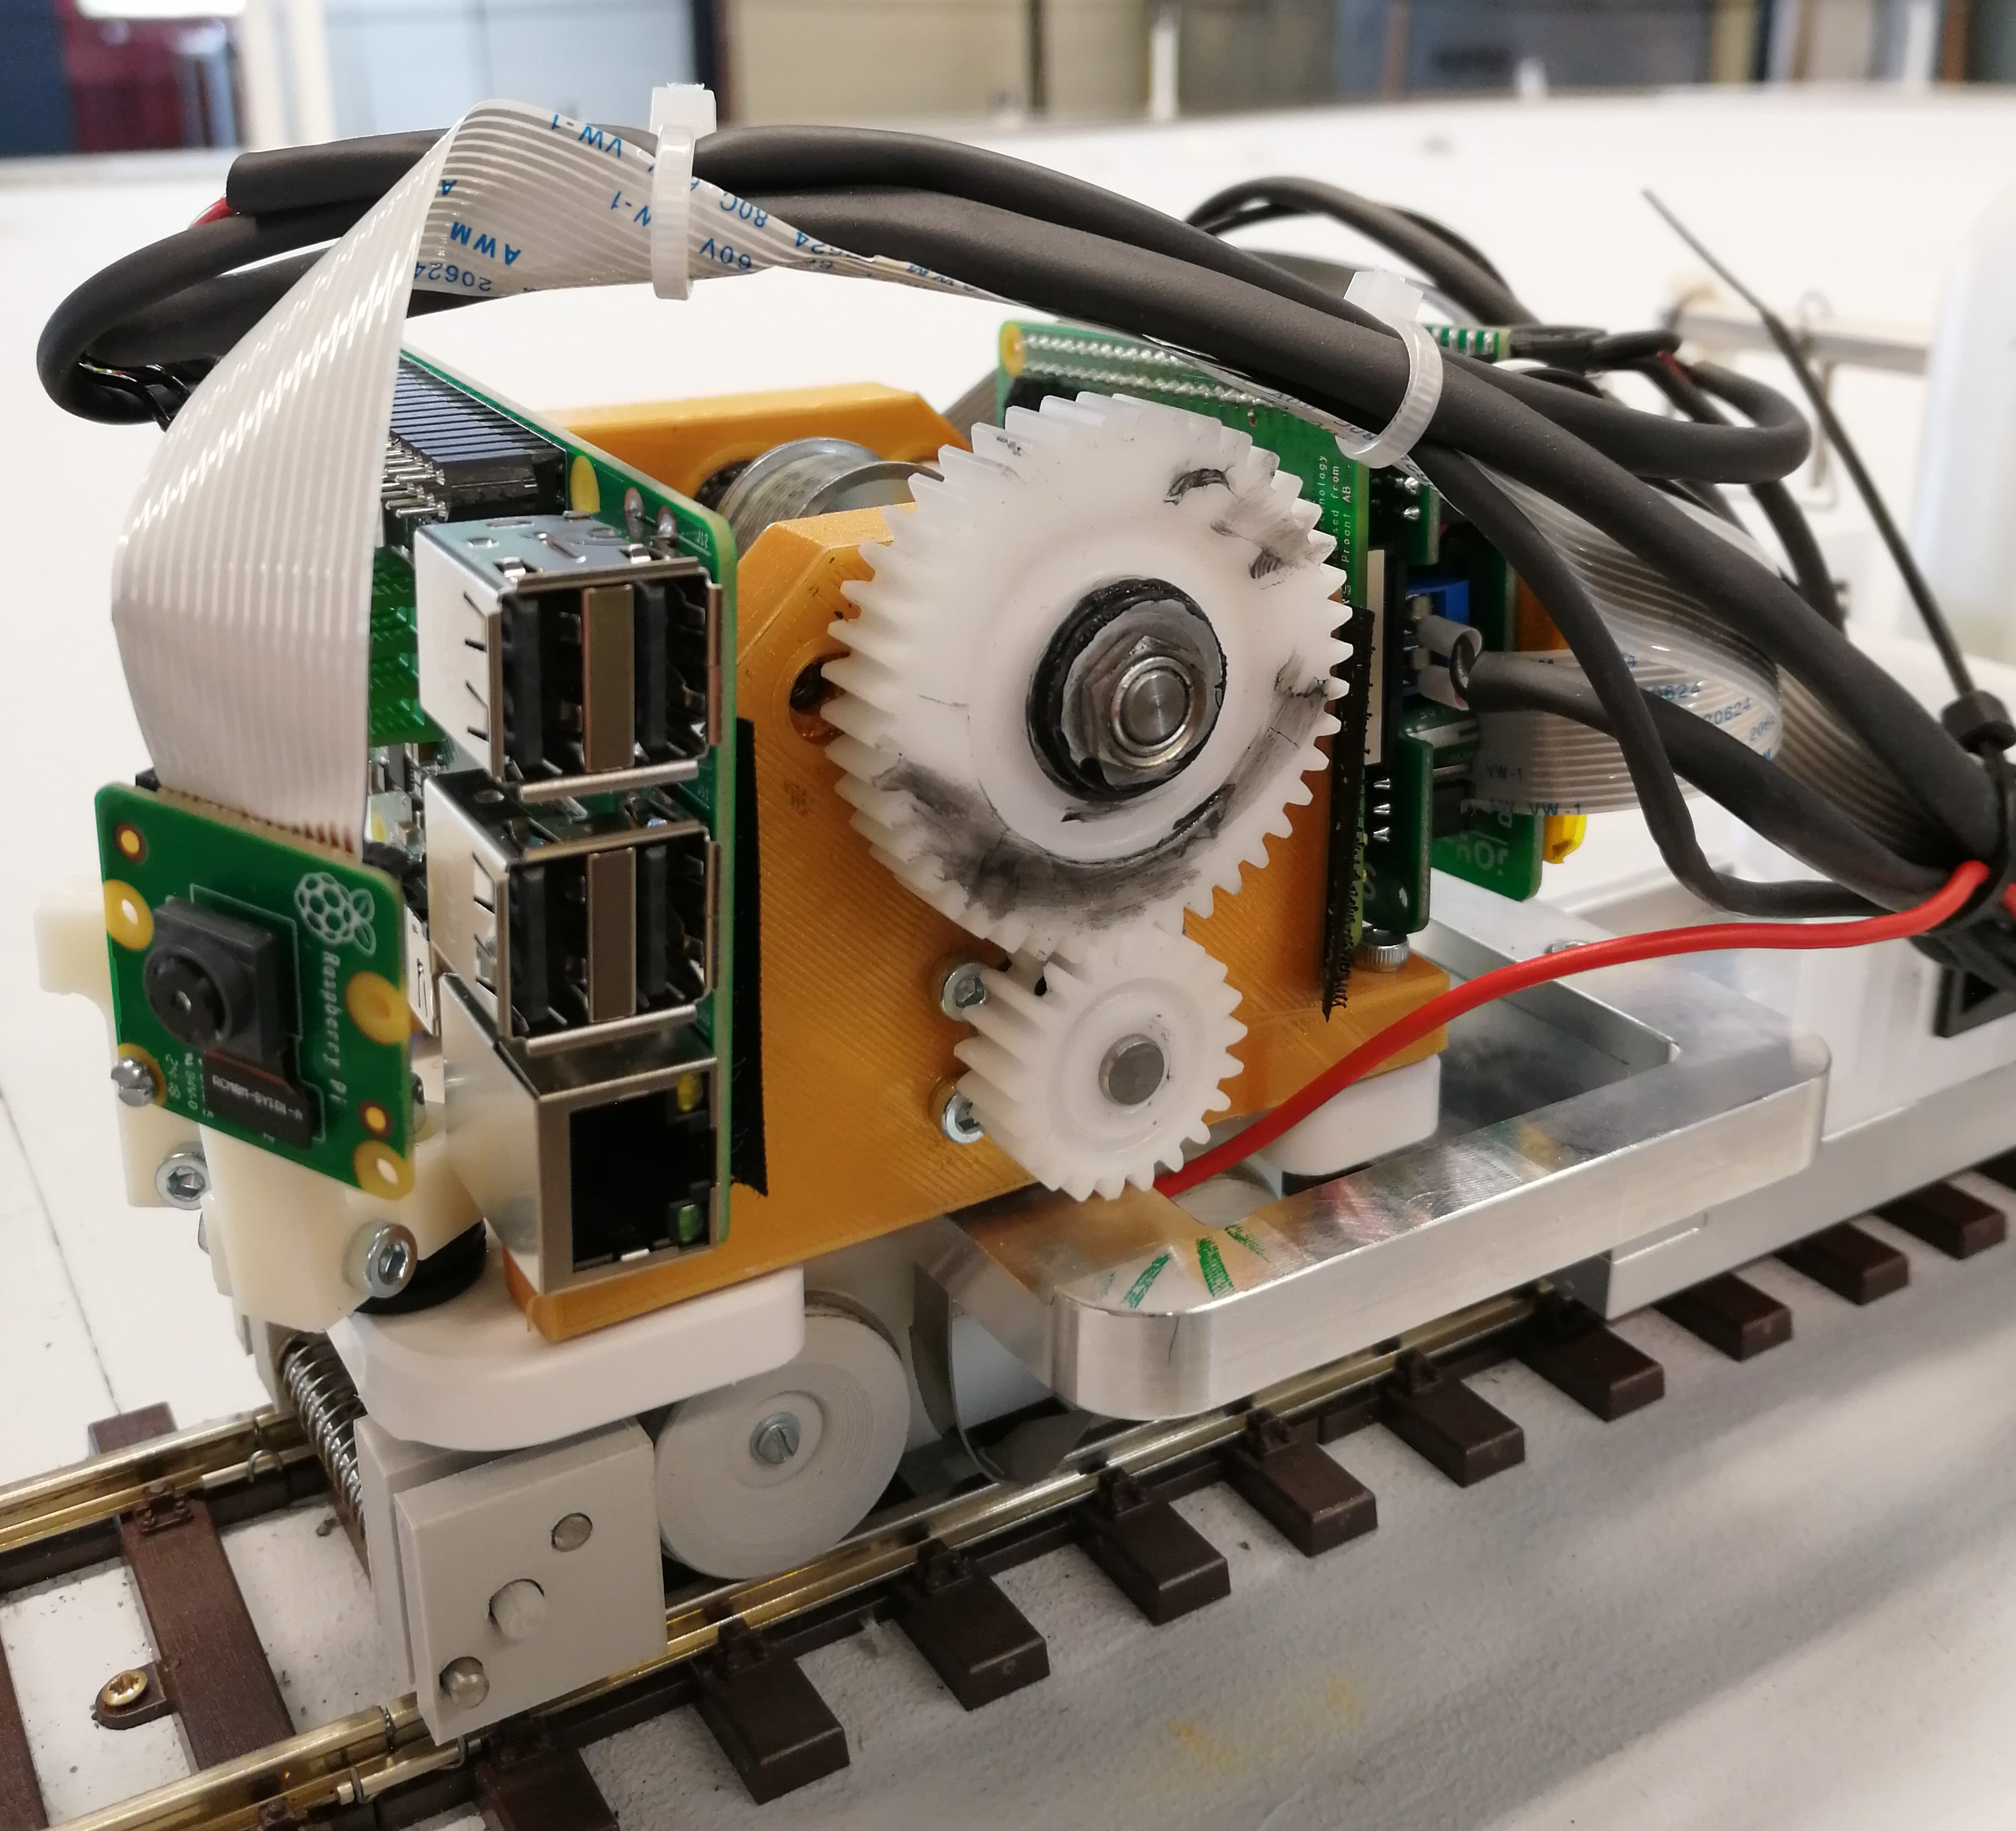
\includegraphics[width=0.48\textwidth]{antriebswagen1.PNG}
  \caption {Antriebswagen}
  \label{fig:antriebswagen3}
\end{figure}

Die Antriebsräder weichen etwas von der geplanten Form ab, da diese mit den O-Ringen nicht wie gewünscht funktioniert. Die O-Ringe weisen den nötigen Reibwert der Räder mit den Gleisen für eine maximale Beschleunigung vor. Der Anpressdruck ist jedoch zu gering, wodurch sich der O-Ring nicht gleichmässig in der Fuge verteilt. Durch ein spezielles Band aus Gummi, welches um das Rad gewickelt ist, wird der gewünschte Effekt erreicht. Bei den Antriebsrädern wie auch bei den Führungsrädern ist der Durchmesser etwas grösser und die Kontur leicht angepasst.\\

\begin{figure}[H]
  \centering
  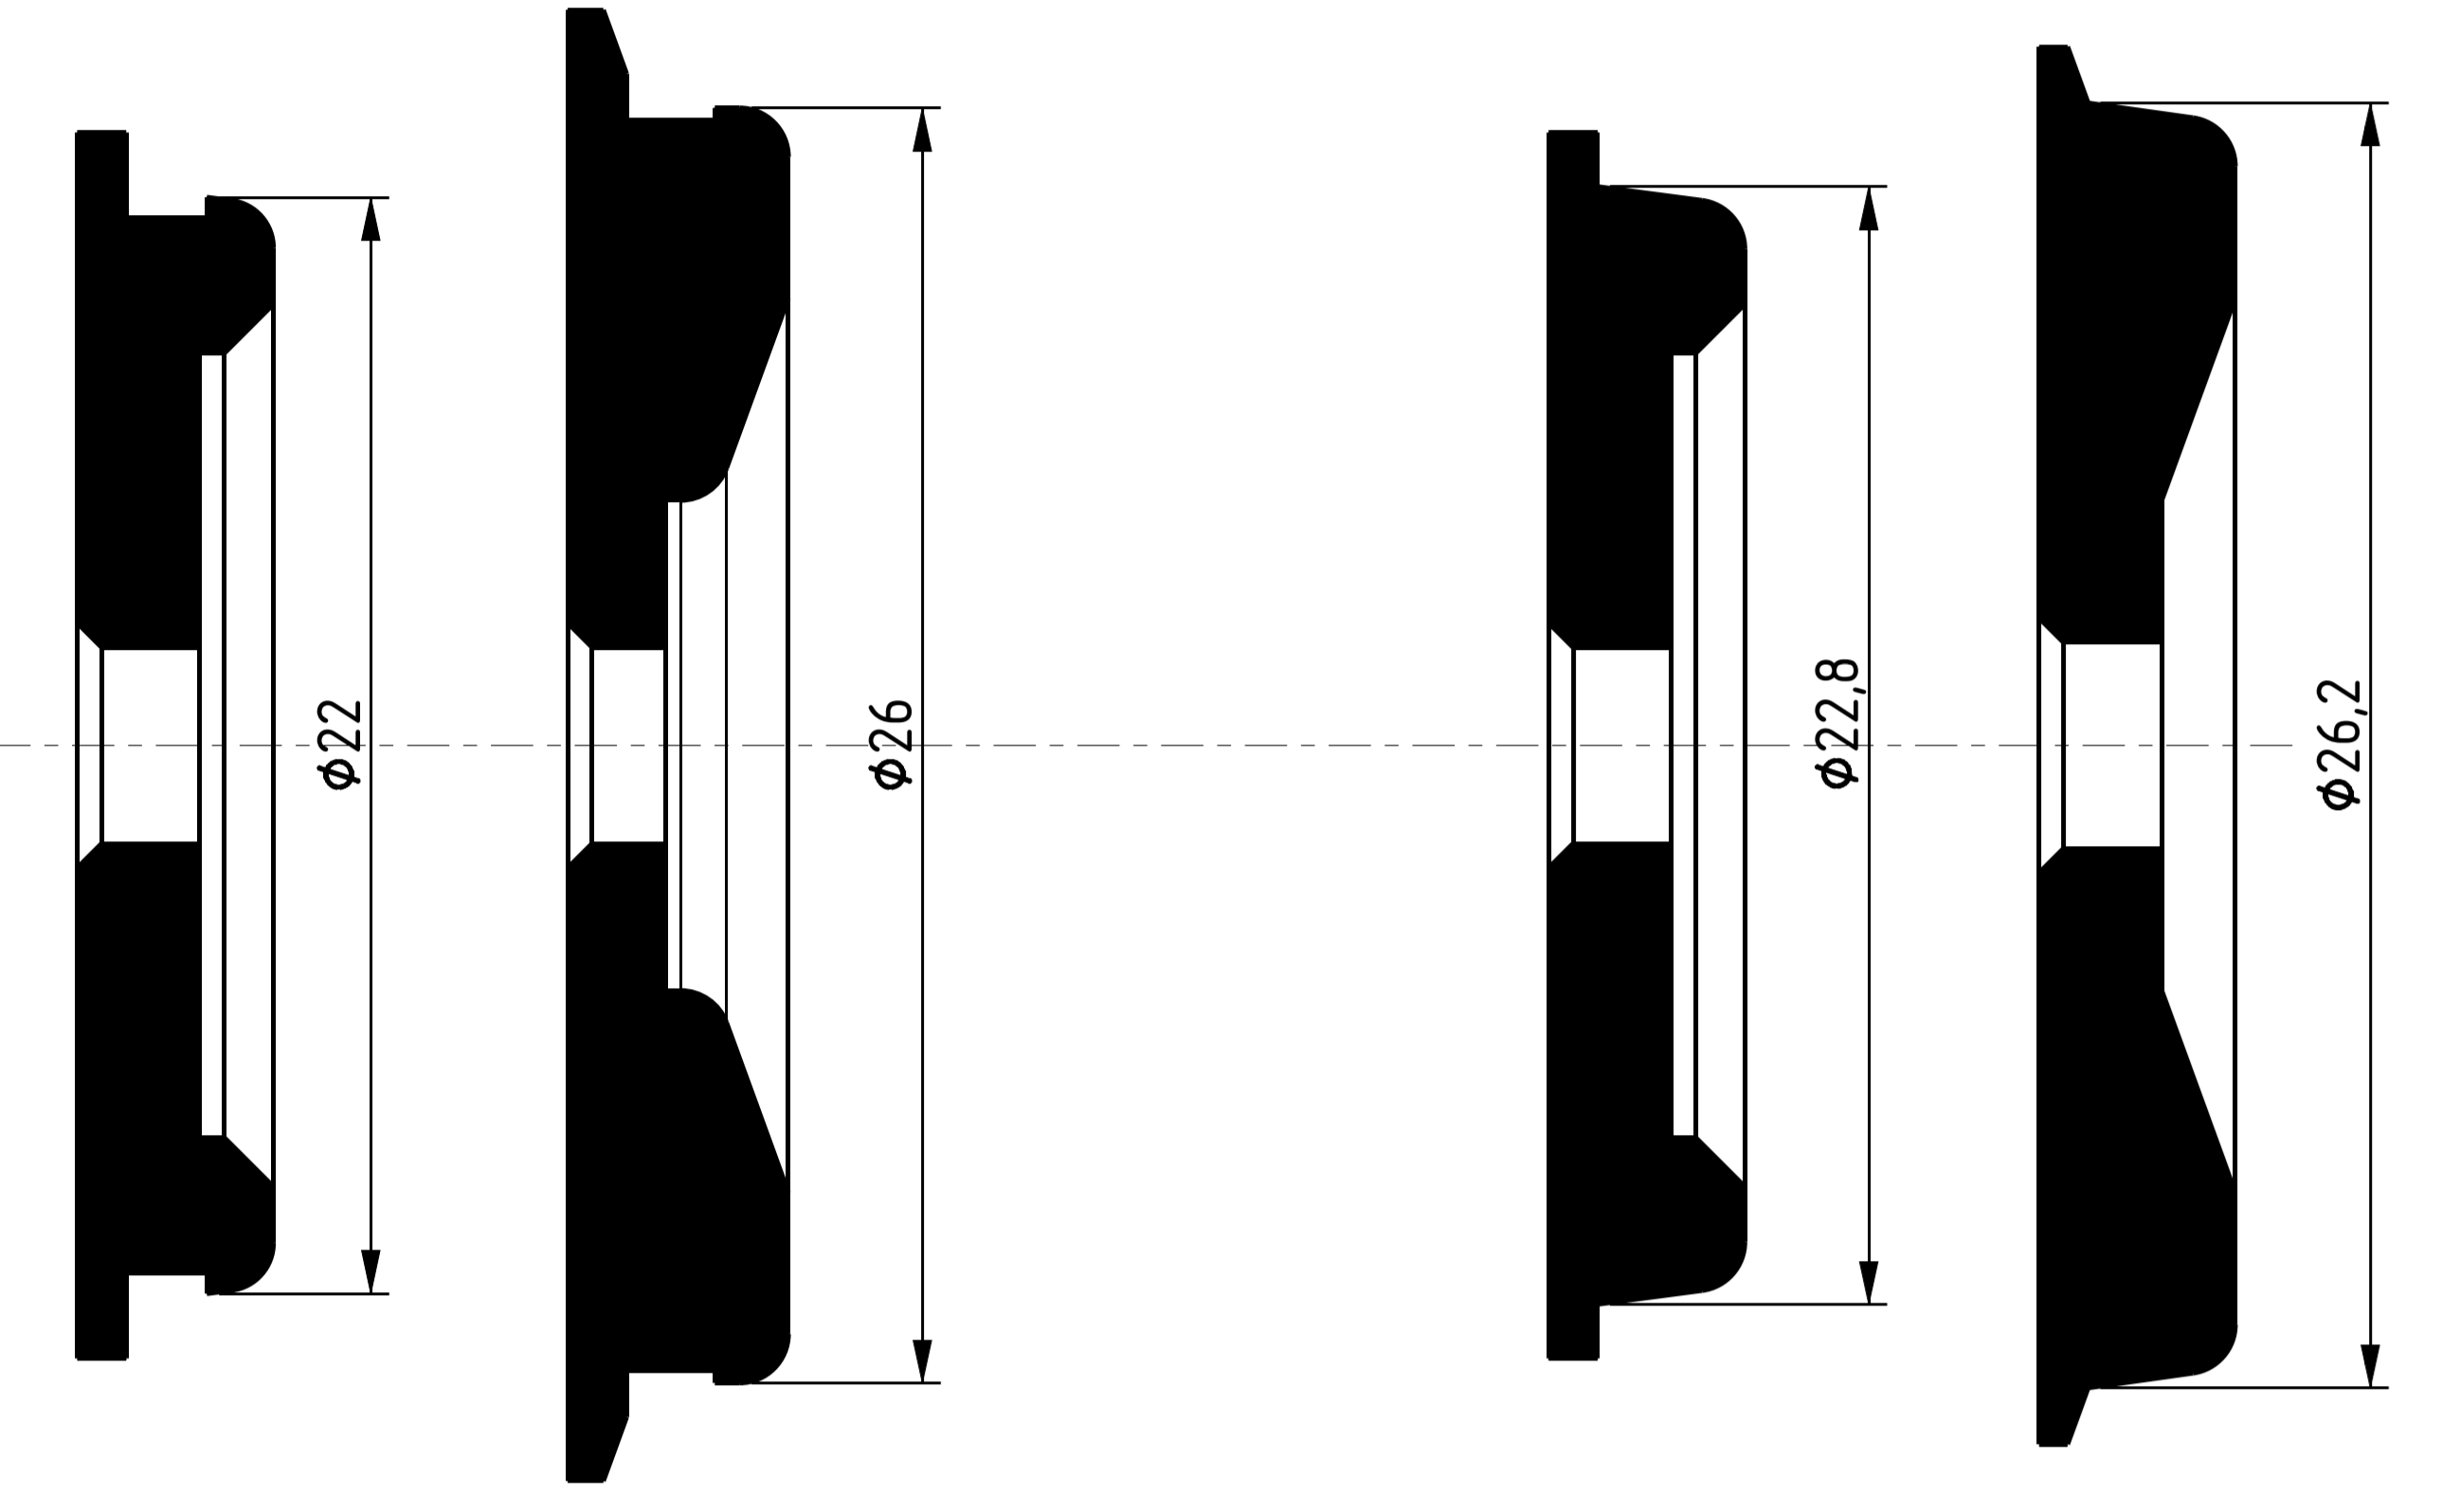
\includegraphics[width=0.6\textwidth]{wagenraeder.PNG}
  \caption {Räder Antriebswagen bzw. Führungswagen - Alt vs. Neu}
  \label{fig:raeder}
\end{figure}

\newpage

\textbf{Maximale Beschleunigung}\\
Der Motor kann gemäss Datenblatt ein maximales Moment von 85.6 mNm erreicht werden. Durch das Übersetzungsverhältnis 2:1 des Getriebes wird ein Moment von 171.2 mNm auf die beiden Radachsen übertragen und somit eine theoretische maximale beschleunigung von 44.79 Meter pro Sekunde im Quadrat erreichen (siehe Tabelle \ref{tab:groessen_beschleunigung}):

$$F_{Rad}=\frac{F_{G}}{8}=\frac{3kg \cdot 9.81m/s^2}{8}=0.375N$$

$$F_{Reibung}=F_{Rad} \cdot k=0.375N \cdot 0.3=0.1125N$$

$$M_{Rad}=M_{Getriebe} \cdot 0.5= 171.2 mNm \cdot 0.5 = 85.6 mNm$$

$$M_{Rad}=F_{Reibung} \cdot a_{max, Getrtiebe} \cdot D_{Rad,Endprodukt} \cdot 0.5$$

$$\boldsymbol{a_{max, Getriebe}}=\frac{M_{Rad}}{\frac{F_{Reibung}}{g} \cdot D_{Rad} \cdot 0.5}=\frac{0.0856Nm}{\frac{0.1125N}{9.81m/s^2} \cdot 0.026m \cdot 0.5}=\boldsymbol{58.53m/s^2}$$\\

\begin{table}[H] \centering
  \begin{tabular}{|l|l|}
  \hline
  \textbf{Grösse} & \textbf{Wert}\\
  \hline
  Durchmesser Rad (Konzept) [D,Konzept]          & 22 Milimeter\\
   \hline
   Durchmesser Rad (Endprodukt) [D,Endprodukt]          & 26 Milimeter\\
   \hline
  Reibungskoeffizient [k]      & 0.3\\
  \hline
  \end{tabular}

  \caption{Grössen für die Beschleunigungsberechnung}
  \label{tab:groessen_beschleunigung}
  \end{table}

Das theoretische maximale Moment beziehungswiese die maximale Drehzahl kann jedoch nicht erreicht werden da diese durch die vorgegebene Speisung beschränkt ist.\\
In der Konzeptphase wurde die theoretische Maximalbeschleunigung gemäss CAD-Daten der Lokomotive (siehe Tabelle \ref{tab:groessen_beschleunigung}) wie folgt berechnet:

$$M_{Rad,Konzept}=F_{Rad} \cdot 0.5 \cdot D_{Rad_Konzept}= 0.1125N \cdot 0.5 \cdot 22mm = 1.24mNm$$
$$M_{Rad,Prototyp}=F_{Rad} \cdot 0.5 \cdot D_{Rad,Endprodukt}= 0.1125N \cdot 0.5 \cdot 26mm = 1.46mNm$$

$$\boldsymbol{a_{max}}=\frac{F_{Reibung}}{\frac{F_{Rad}}{g}}=\frac{0.1125N}{\frac{0.375N}{9.81m/s^2}}=\boldsymbol{2.94m/s^2}$$
\\

Bei den Probefahrten auf der vorgebenen Teststrecke (siehe Abschnitt "Teststrecke") hat sich eine maximale Beschleunigung von ... herausgestellt. Diese ergibt sich durch das Moment welches über das Getriebe auf die Räder übertragen wird, die Normalkraft des Zuges und der Reibwert zwischen Räder und Gleis. Dieser Wert entstand durch Messungen mit einem Beschleunigungsensor.\\

\newpage

\textbf{Maximale Geschwindigkeit}\\
Die Maximale Geschwindigkeit in der Kurve wurde in der Theorie mit den gegebenen Grössen (siehe Tabelle \ref{tab:geschwindigkeitsberechnung}) folgendermassen berechnet:\\

\begin{table}[H] \centering
    \begin{tabular}{|l|l|}
    \hline
    \textbf{Grösse} & \textbf{Wert}\\
    \hline
    Minimaler Radius  [r]                               & 0.8 Meter\\
     \hline
    Masse [m]                                           & 3 Kilogramm\\
    \hline
    Schwerpunkt in x-Achse (maximaler Wert) [x]         & 0.0225 Meter\\
    \hline
    Schwerpunkt in y-Achse (maximaler Wert) [y]         & 0.05 Meter\\
    \hline
    \end{tabular}

    \caption{Grössen für die Geschwindigkeitsberechnung}
    \label{tab:geschwindigkeitsberechnung}
    \end{table}

Die Gewichts- und Zentripedalkraft, welche das Gleichungssystem für die Geschwindigkeitsberechnung bilden, sind wie folgt definiert:

$$F_{G}=m \cdot g=3kg \cdot 9.81m/s^2=29.4N$$

$$F_{max, z}=\frac{F_{G} \cdot x}{y}=\frac{29.4N \cdot 0.0225m}{0.05m}=13.24N$$

\begin{figure}[H]
    \centering
    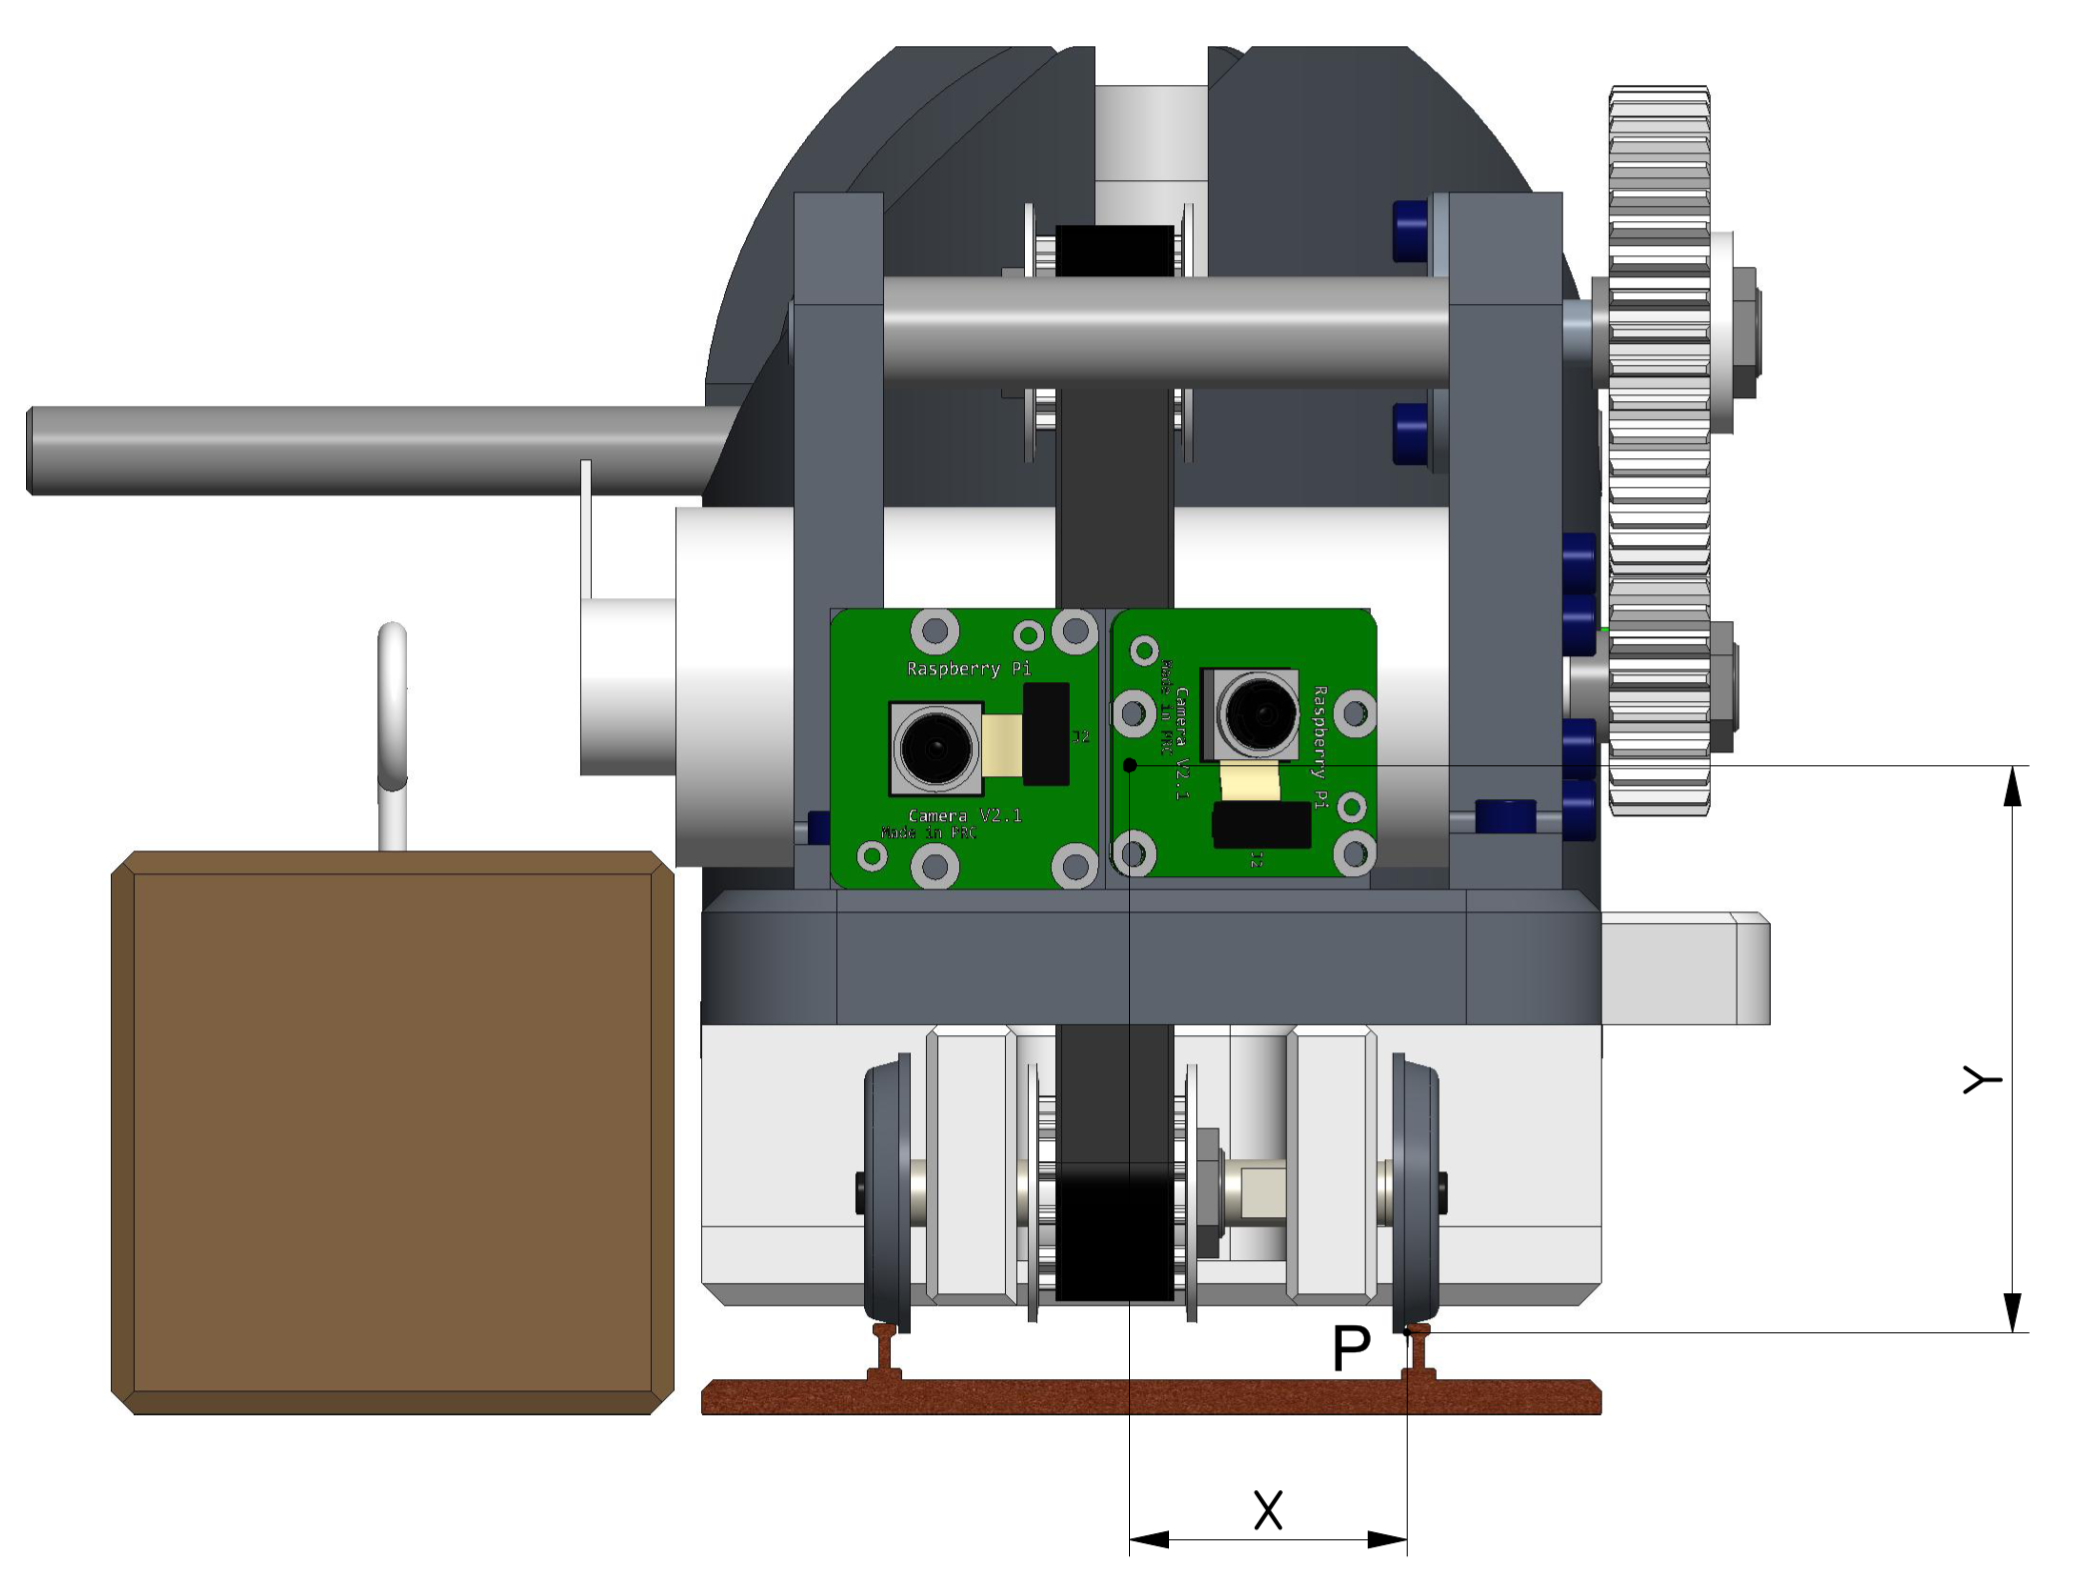
\includegraphics[width=0.6\textwidth]{schwerpunkt.PNG}
    \caption {Schwerpunkt der Lokomotive}
    \label{fig:schwerpunkt}
\end{figure}

Da das Drehmoment eine vektorielle Grösse ist, müssen die beiden entstehenden Momente am Drehpunkt ''P'' am Gleis zusammen Null ergeben (siehe Abbildung \ref{fig:schwerpunkt}). Oder anders gesagt, müssen die beiden Momente gleich gross sein, damit das System ''statisch'' bestimmt ist. Die Berechnungen sind auf den kleinsten Kurvenradius ausgelegt, da dort die grösste Zentripedalkraft entsteht. Somit ergibt sich eine maximale Geschwindigkeit von 1.53 Meter pro Sekunde:

$$F_{max, z}=\frac{m \cdot v_{max}^2}{r};\boldsymbol{v_{max}}=\sqrt\frac{F_{max, z}\cdot r}{m}=\sqrt\frac{13.24N \cdot 0.8m}{3kg}=\boldsymbol{1.53m/s}$$\\

Gemäss den Messungen auf der Teststrecke ist eine maximale Geschwindigkeit von 2.2 Meter pro Sekunde erreichbar. Der limitierende Faktor ist nicht das Kippen beziehungseise entgleisen in der Kurve, sondern der Motor. Der Motor erreicht dieser Geschwindigkeit seine maximale Leistung mit den gegebenn Werten des Stromes und der Spannung. Somit fährt die Lokomotive 1.7 Meter pro Sekunde schneller als im Anforderungskatalog deklariert wurde und etwa 0.7 Meter pro Sekunde schneller als der theoretisch berechnete Wert. An Hand dieser Ergebnisse ist ersichtlich, dass der Schwerpunkt optimaler liegt, als angenommen wurde und zusätzlich die Kurvenvorrichtung dazu beiträgt, dass die Lokomotive in der Kurve schneller fahren kann.\\

\textbf{Befestigung der Elektrokomponenten}\\
Der Montageraum für die Elektrokomponenten ist beim Endprodukt nicht nur auf dem Führungswagen, sondern ebenfalls auf dem Antriebswagen. Auf dem Antriebswagen sind Elektrokomponenten mit Klett an der Antriebseinheit befestigt. Weiter sind Elektrokomponenten wie Buzzer oder Näherungssensor an den Freien Flächen der Lokomotive angebracht. Auf der Abbildung \ref{fig:elektrokomponenten} sind die montierten Elektorkomponenten und deren Verkablung ersichtlich.\\

\begin{figure}[H]
  \centering
  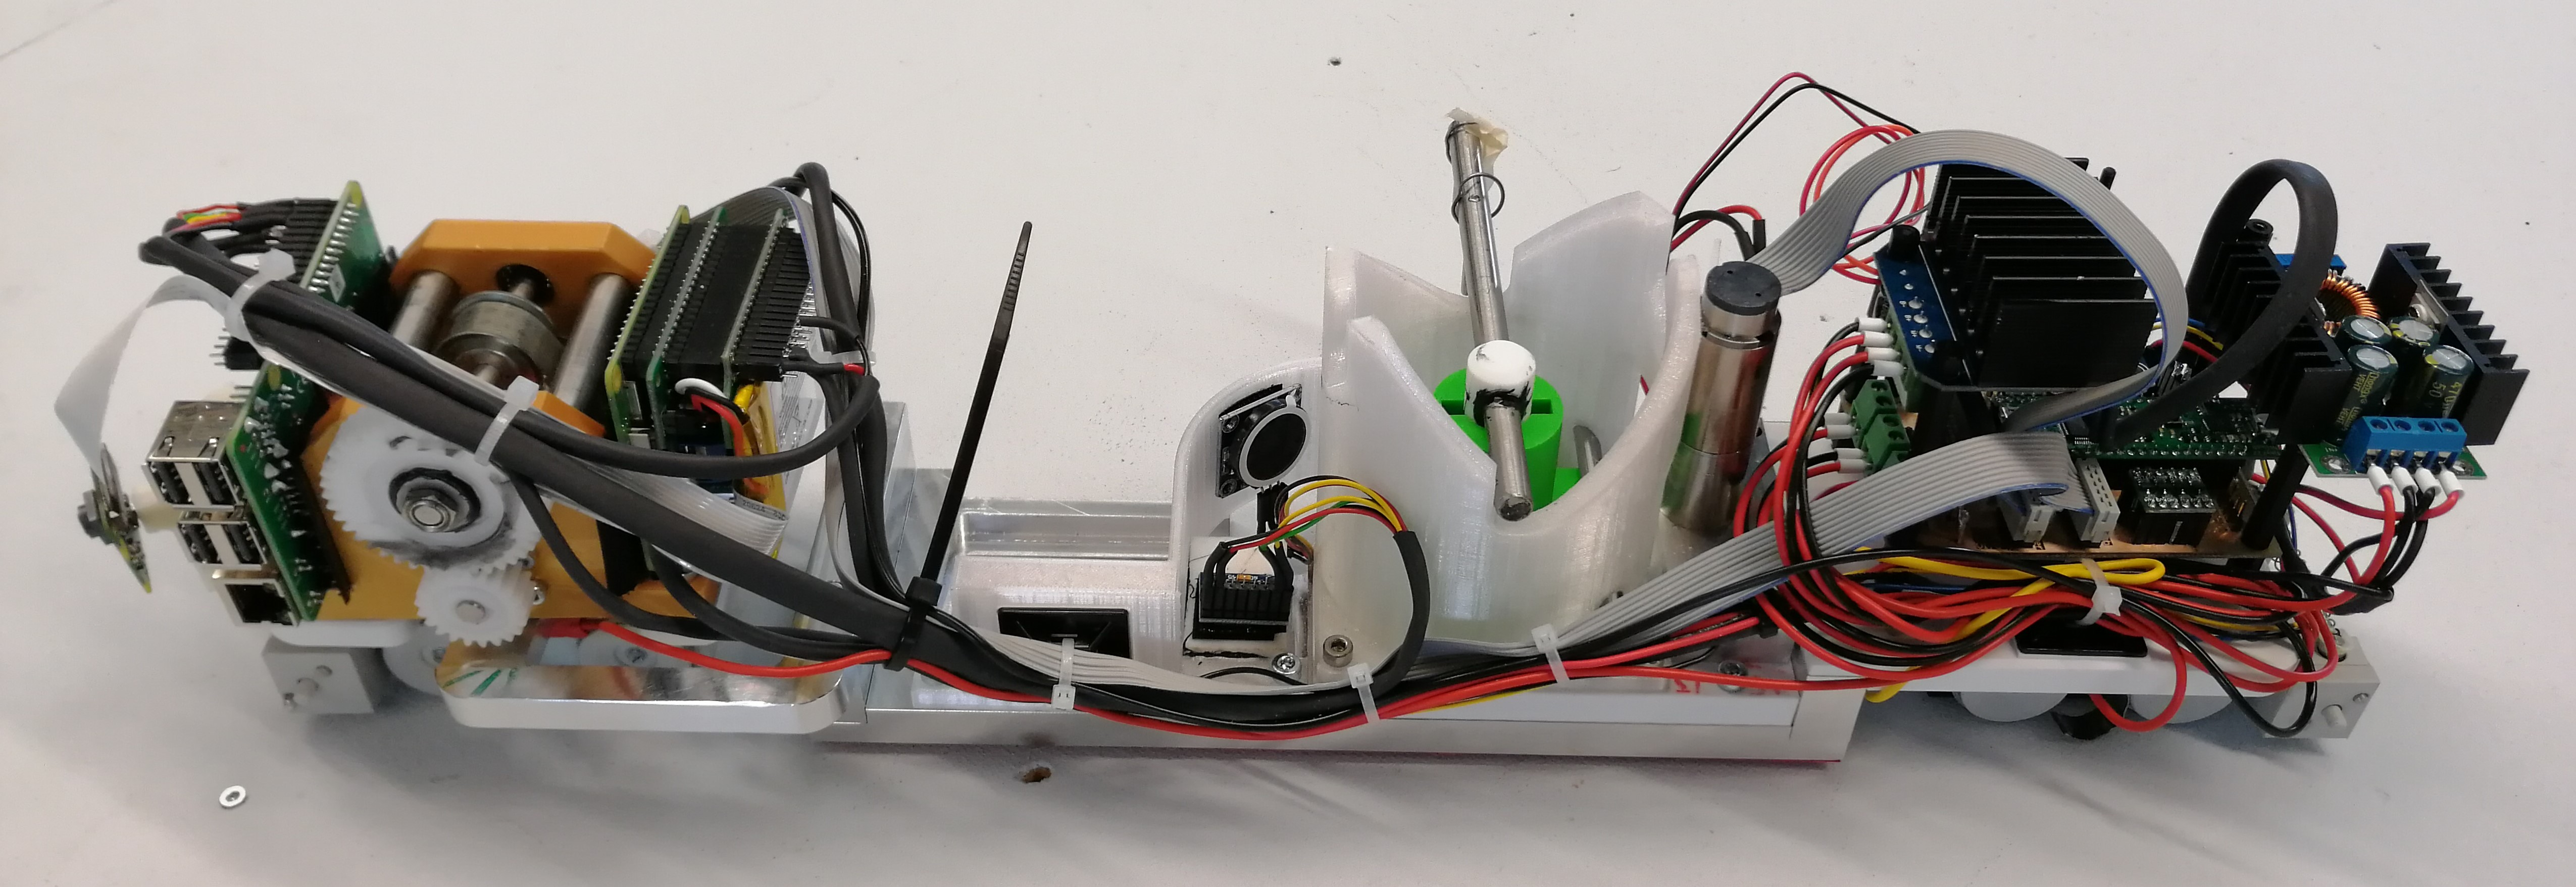
\includegraphics[width=1\textwidth]{lokomotive3.PNG}
  \caption {Elektrokomponenten}
  \label{fig:elektrokomponenten}
\end{figure}

\begin{figure}[H]
  \begin{minipage}{.5\textwidth}
    \textbf{Stromabnahme}\\
    Die anfänglich konzipierten Schleifkontakte (siehe Abbildung \ref{fig:schleifkontakte}) gebogen aus Federstahl erweisen sich als eine einfache und zuverlässige Art der Stromabnahme. Für die ersten Testfahrten wurde eine Stromabnahme am hinteren Wagen, dem Führungswagen, angebracht. Es wurde jedoch festgestellt, wenn Unebenheiten der Strecke vorhanden sind, die Möglichkeit eines Kontaktverlustes besteht. Somit wurde in einem zweiten Schritt eine zweite Stromabnahme am Antriebswagen befestigt, welche diese Gefahr minimert.\\
   \end{minipage}
  \begin{minipage}{.5\textwidth}
    \flushright
    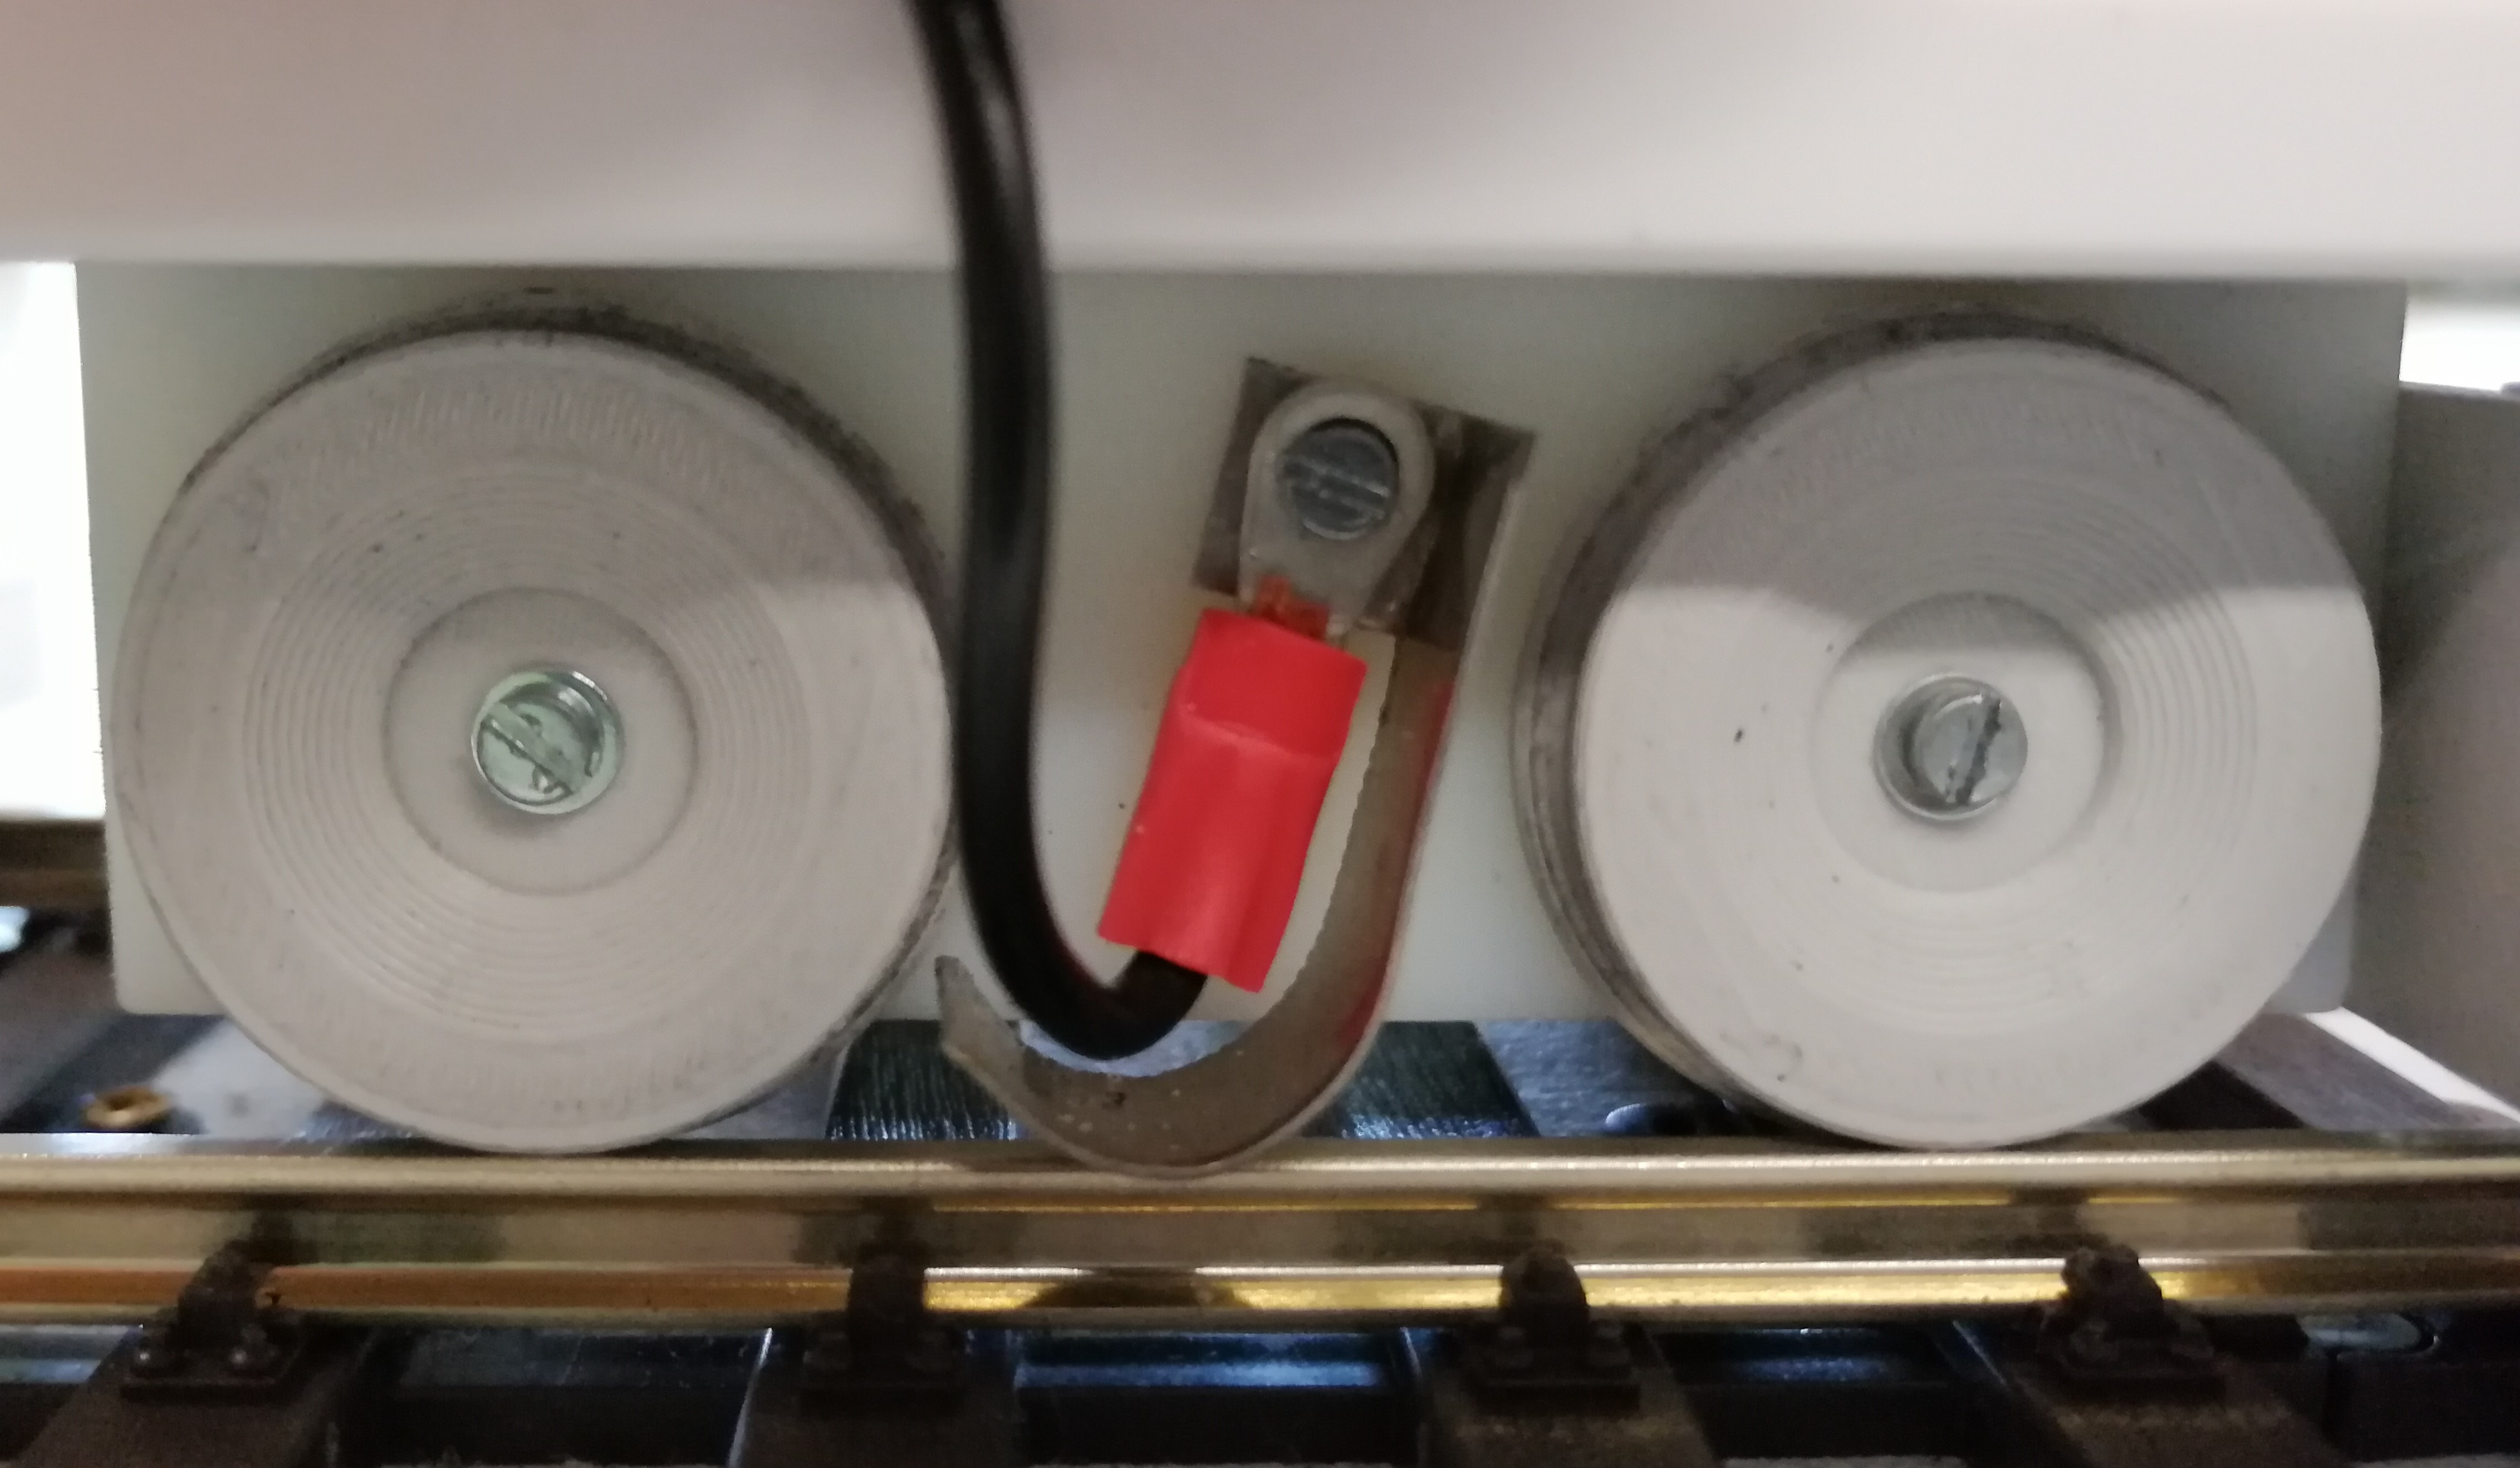
\includegraphics[width=0.9\textwidth]{schleifkontakt.PNG}
    \caption {Schleifkontakte}
    \label{fig:schleifkontakte}
    \end{minipage} 
\end{figure} 

\newpage

\subsection{Ergebnisse aus Versuchen und Tests}

\textbf{Teststrecke}\\
Die grösste Herausforderung an das Fahrwerk besteht bei einer Doppelkurve mit engem Radius (siehe oben mitte in Abbildung \ref{fig:teststrecke1}). Ansonsten erfüllt die Lokomotive die Anforderungen an die Strecke. Sie berührt das Lichtraumprofil und kein anderes Element auf der Testrecke, mit einer Ausnahme, dem Holzwürfel. Ein Problem für die Mechanik stellt die enge Doppelkurve dar, da dadurch grosse Kräfte an der Lokomotive entstehen, welche aber durch die Kurvenführung weitgehen behoben wird.\\

\begin{figure}[H]
    \centering
    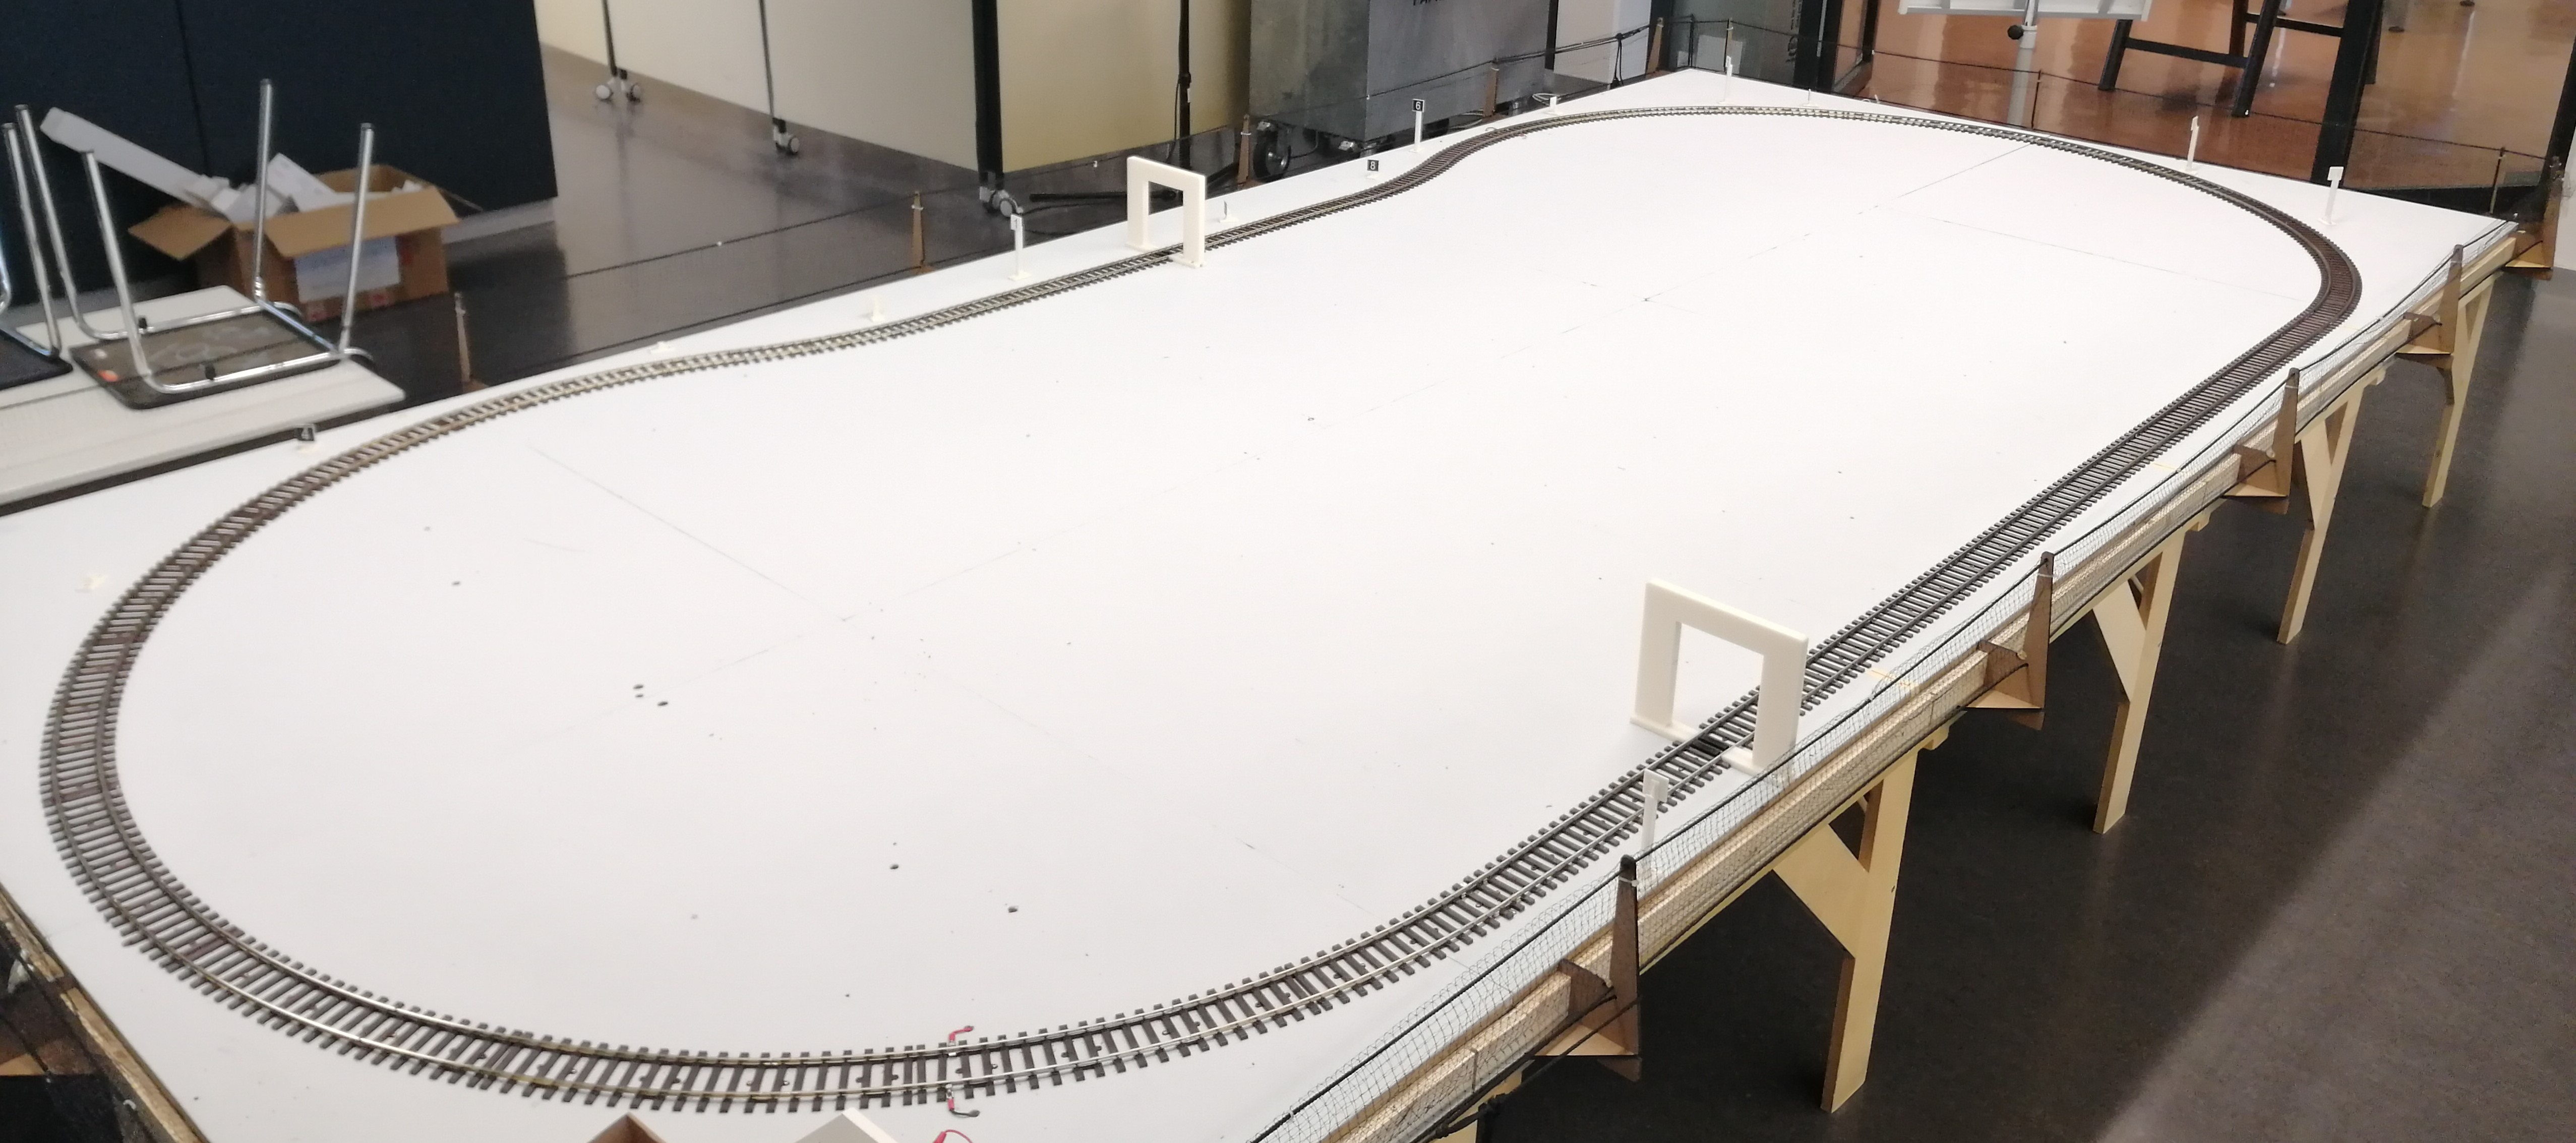
\includegraphics[width=0.8\textwidth]{teststrecke1.PNG}
    \caption {Aufbau Teststrecke}
    \label{fig:teststrecke1}
  \end{figure}

\textbf{Wagenräder}\\
Die Räder der Lokomotive sind für zwei Bereiche vorgesehen. Einerseits gibt es Räder für den Antriebswagen und andererseits solche für den Führungswagen. Die Räder für den Fürhungswagen haben im Gegensatz zu denen des Antriebswagens keine spezielle Bearbetiung. In einem ersten Veruch wurden die Reifen mit einem O-Ring versehen. Da der Anpressdruck durch das Gewicht der Lokomotive zu gering war und die Fuge nicht gleichmässig mit der Gummimasse gefüllt wurde, kippte der Zug leicht auf den Gleisen hin und her, da zusätzlich der Absatz für die Führung zu kurz war. In einem nächsten Schritt wurde ein Gummispray Schicht für Schicht auf die Räder gesprayt. Jedoch weissten diese bei der Testfahrt bereits grossen Verschleiss auf und ist somit für die Forderung nicht ausreichend. Als letzter und funktionsfähiger Versuch wurden die Räder mit einem speziellen Gummiband umwickelt. Die Funktion ist erfüllt und der Verschleiss hält sich in einem vernünftigen Rahmen.

\textbf{Stromabnahme}\\
In einem ersten Versuch wurde die Stromabnahme nur an einem Ort, dem Führungswagen, abgenommen. Jedoch ist die Gefahr gross, dass die Schleifkontakte bereits bei kleinsten Unebenheiten der Strecke den Kontakt verlieren und das System zum Absturz bringen. Somit wurden zusätzlich zwei Schleifkontakte am Antriebswagen befestigt, welche die Gefahr minimiert. Die Stromabnahme funktioniert nun mit der gewünschten Zuverlässigkeit.

\textbf{Kurvenführung}\\
Die Kurvenführung wurde in mehreren Testfahrten getestet und zeigte die gewünschten Effekte auf. Lediglich die Feder beziehungsweise die Federrate musste angepasst werden, damit der Anpressdruck der Stahlstifte genügend hoch ist und so der Zentripedalkraft der Lokomotive entgegenwirken kann.

\end{document}